\chapter{Observational data}\label{chp:obs}
The main observational data used within this thesis are of four different kinds: precipitation, discharge, flood extent and terrain elevation. Due to the different peculiarities of each variable, they are treated separately in the following sections. \Cref{sec:pr_obs} will give an overview of precipitation datasets available over the study domain, including a brief analysis of precipitation uncertainty employing eight different datasets (\cref{sec:uncertainty_pr}). \Cref{sec:disch_obs,sec:flood_obs} will describe the available discharge and flood observations, while in \cref{sec:DEM} the choice of Digital Elevation Model for the subsequent hydrological and hydraulic simulations will be discussed.

%------------------------------------
%	PRECIPITATION OBS
%------------------------------------
\section{Precipitation observations} \label{sec:pr_obs}
Precipitation is probably the most difficult of all atmospheric climate variables to measure reliably, due to the huge spatio-temporal variability (especially in summer) and to the physical difficulty of setting up and maintaining a dense network of high-maintenance sensors. In our multi-model approach (see \cref{sec:3_mod_apprach}), however, it is vital that the precipitation input data is of sufficient quality and resolution to provide information even about very local, fast thunderstorms, which can trigger flooding in smaller catchments. Moreover, it is important to analyse the longest time series possible, so that rare events, which by definition have a long Return Period, can be properly represented.

In this project, precipitation observations are utilised for calibration, for validation and for driving the hydrological model CHyM (see \cref{sec:chym}).
  
\subsection{Types of precipitation measurements} \label{sec:types_pr_meas}
Precipitation measurements come from essentially three distinct sources:
\begin{description}
    \item[In-situ] Station observations are widely regarded to be the most reliable source of information for precipitation observations \citep{Hughes2006}. Several types of rain gauges exist, with the most common type of instrument being the \emph{tipping bucket rain gauge} (\cref{fig:tipping_bucket}). It consists of a small bucket of fixed size which fills up with precipitation and mechanically tips and empties, triggering a counting switch, every (usually) \SI{0.1}{\milli\metre} of rain. The buckets are usually heated, so that solid precipitation (snow, ice) is melted and correctly registered. Having moving parts means that most in-situ precipitation stations require constant and attentive maintenance, as ill-maintained sensors can easily get stuck (see \cref{fig:ts_rain/a} for an example). In general, in-situ precipitation measurements suffer greatly from the problem of gauge undercatch (see \cref{sec:gauge_undercatch}), in which, due to strong winds, a smaller amount of precipitation than expected enters the measuring funnel. In-situ data usually offer the longest time-series of all precipitation measurements techniques, with some datasets reconstructing rainfall back to the 19th century: the HISTALP project \citep{Auer2007}, for example, provides rainfall on the Alpine range using data as old as the 1800; \citep{Brunetti2006} goes as far as 1750 with monthly precipitation data over Italy. Uncertainties in in-situ data are mostly related with low station density and choice of gridding technique, so that different datasets can have significantly different climatology, especially in areas of low data availability \citep{Prein2017}. Additional details on station-based precipitation datasets, such as E-OBS and EURO4M-APGD, can be found in \cref{sec:obs_datasets}.
    \item[Ground radar] Available since the mid ’80s, ground radar observations are obtained from data on the reflectivity of the atmosphere. Rain and water vapour reflect radar waves, and the analysis of this effect allows for estimation of precipitation and wind speed; however, the displayed data can differ from the rainfall actually measured at the surface by in-situ gauges, especially in areas of complex topography, where the radio waves can easily be shielded or reflected by mountain ranges \citep{Germann2006, Wuest2010}. On the other hand, the time and space resolution of radar-based datasets cannot be matched by in-situ data. Overall, radar observations are primarily used for weather prediction and analysis and for studying specific events \citep[e.g.][]{Bertato2003}, but are sometimes also used as a tool for filling or extending other kinds of measurements.
    \item[Satellite] Space-borne precipitation measurements \citep[see][for an overview]{Kidd2011} have been available since the mid ’70s and have been on the rise in both availability and reliability ever since. Much like radars, they scan the atmosphere with several frequencies (microwave and radio), and interpret the reflected waves according to specific algorithms. Their main advantage is the relatively high resolution and very large coverage, being available even in regions where no station or radar is in place. However, the physical limitations, different measurement techniques and algorithms used to retrieve precipitation from interferometry data introduce large uncertainties \citep{Sarachi2015, Maggioni2016, Bartsotas2018, Tian2010, Bytheway2013}. Large advancements have occurred in satellite-based precipitation measurements since the early days of remote sensing from space, and there is no doubt that this data source is essential for global datasets; it is however generally found and agreed upon \citep{Rossi2017, Prein2017, Gao2013, Bowman2005} that in regions where in-situ data is available (such as most of Europe) station-based datasets still provide more reliable data. Examples of global satellite-based precipitation datasets are PERSIANN, CMORPH, TRMM, GPCP and GPM (see \cref{tab:prec_obs_ita} for citations).
\end{description}

\begin{figure}
    \centering
    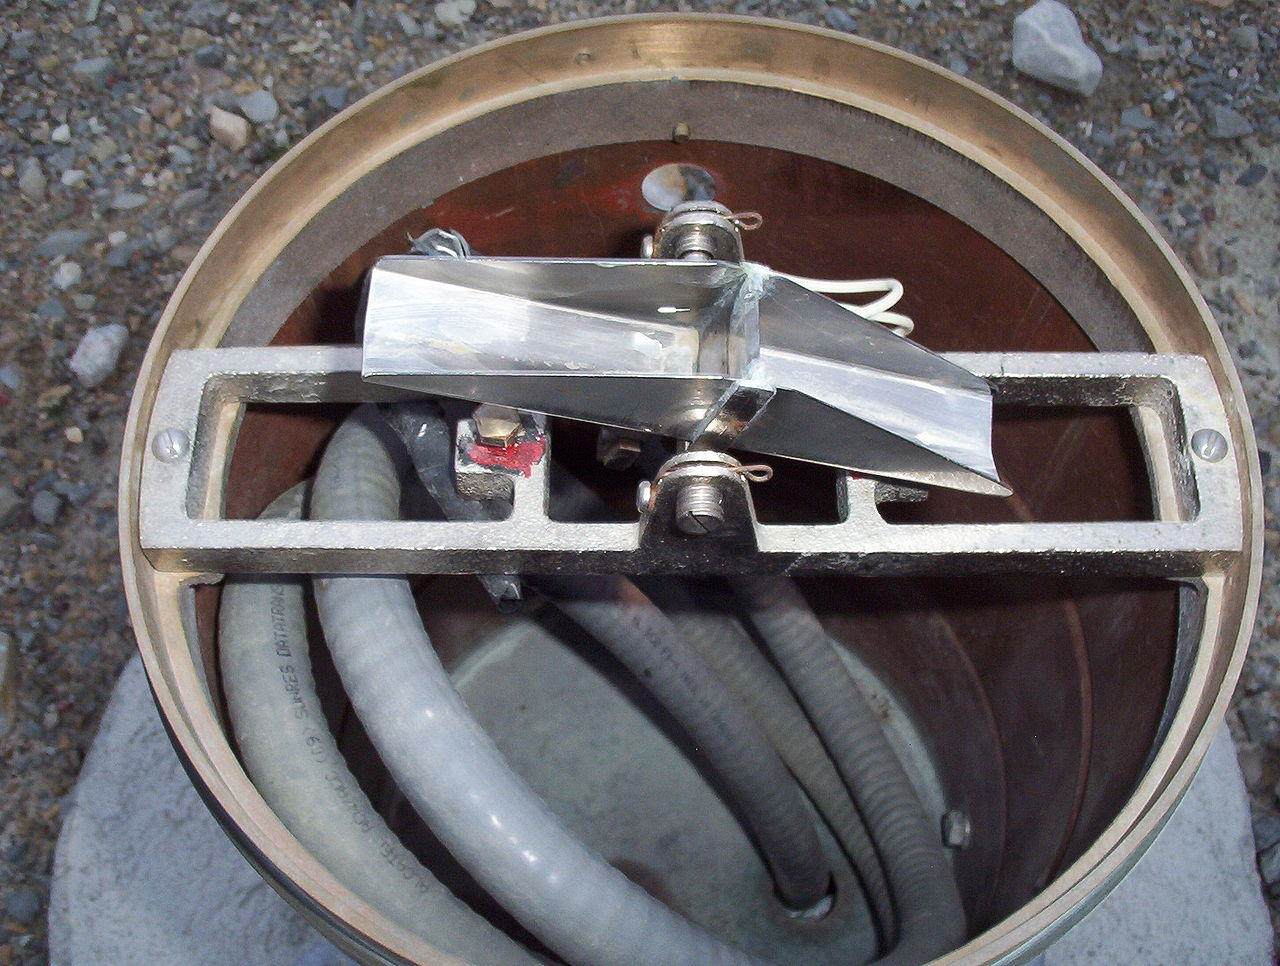
\includegraphics[width=0.7\textwidth]{figures/tipping_bucket}
    \decoRule
    \caption[Tipping bucket rain gauge]{A tipping bucket rain gauge, the most common type of precipitation measuring instrument,  with the buckets exposed.}
    \label{fig:tipping_bucket}
\end{figure}

\subsection{Gauge undercatch} \label{sec:gauge_undercatch}
The main source of uncertainty for in-situ precipitation observations is the phenomenon of \emph{gauge undercatch}. This term indicates the underestimation of precipitation due to local turbulent effects around the gauge caused by the wind interacting with the sides of the instrument, as seen in \cref{fig:undercatch}. Gauge undercatch is hard to quantify, but it can severely impact the measurements of precipitation, especially for solid precipitation in windy days. According to some studies, underestimation of total precipitation can be as high as \SIrange{30}{40}{\%} for some winter stations \citep{adam2003Adjglogripresysbia, Isotta2014, Kochendorfer2017a}, with peaks of 80\% in some cases \citep{Kochendorfer2017, Wolff2015}. 
Shielded gauges, in which the collector is partially shielded from the wind (see \cref{fig:gauges}), reduce, but do not eliminate this problem \citep{Duchon2001}.\\
Correcting precipitation datasets for gauge undercatch is possible, but detailed information about local station exposure and sensor type are necessary to perform reasonable estimates \citep[see e.g.][]{Johansson2002, Mohr2009, Adler2018}.
In the Norwegian observational dataset created by \citet{Mohr2009}, for example, the correction method from \citet{Forland1996}, is applied: each station is associated with an exposure index, and a correction factor ranging from 1.02 to 1.8 (depending on precipitation type and exposure) is applied.
Observational datasets which are produced through data assimilation via a meteorological model \citep[see e.g.][]{Vidal2010, Landelius2016} often implicitly include correction factors.\\
Due to the complexity and variability of the datasets used through this thesis, and especially for the dataset described in \cref{chp:itaobs}, no attempt at correcting for gauge undercatch was performed.

\begin{figure}
    \centering
    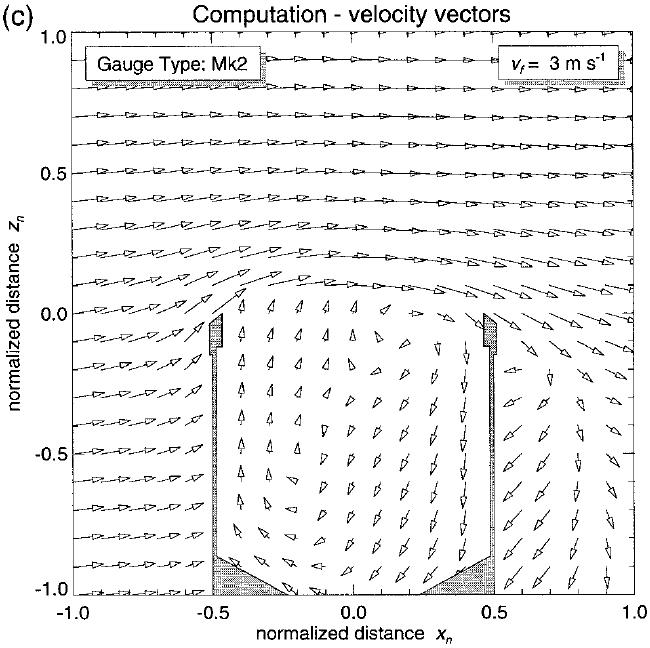
\includegraphics[width=0.7\textwidth]{figures/undercatch}
    \decoRule
    \caption[Gauge undercatch theoretical example]{Wind velocity vectors around an unshielded gauge. Wind blowing precipitation away from the collector is the main cause of gauge undercatch. From \citet{Nespor1999}.}
    \label{fig:undercatch}
\end{figure}

\begin{figure}
    \centering
    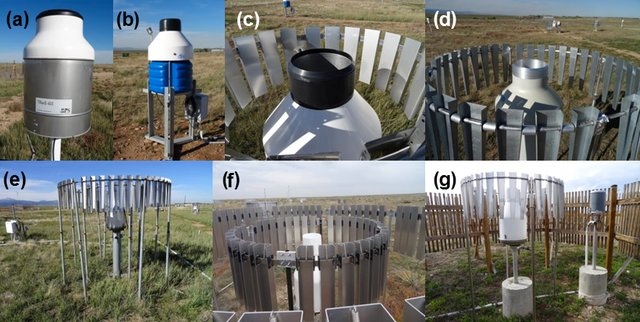
\includegraphics[width=\textwidth]{figures/gauges}
    \decoRule
    \caption[Shielded and unshielded rain gauges]{7 different rain gauges. a) and b) are unshielded, the rest show an array of different shielding methods. From \citet{Kochendorfer2018}.}
    \label{fig:gauges}
\end{figure}

\subsection{Precipitation datasets available over Italy} \label{sec:obs_datasets}
\Cref{tab:prec_obs_ita} lists some of the currently available gridded precipitation datasets covering the Italian territory.
Two high-resolution, high-quality precipitation datasets for the Alps and Northern Italy (EURO4M-APGD and ARCIS) are available for a long observational period (38 and 55 years respectively); Central and Southern Italy, however, are only covered by European-wide and World-wide datasets, such as E-OBS, CHIRPS and the HMR reanalysis. In \cref{sec:uncertainty_pr}, a few of these datasets will be compared.\\
Of those listed in \cref{tab:prec_obs_ita}, only three high-resolution datasets provide sub-daily accumulations (PERSIANN-CDR, GPM and the UERRA reanalysis); of these, the PERSIANN-CDR reanalysis has been shown to perform poorly over Europe \citep{Prein2017}, GPM is available only since 2014, and UERRA-HARMONIE is a relatively new reanalysis which has so far seen little use and validation.
The precipitation dataset described in \cref{chp:itaobs} thus represents, to the author's knowledge, the first attempt at creating a sub-daily precipitation dataset deriving from in-situ observations specifically for the Italian territory.

% \begin{sidewaystable}[]
% \centering
% \begin{tabular}{@{}m{2.2cm}m{1.9cm}m{1.8cm}m{1.2cm}m{1.7cm}m{2.2cm}m{6cm}m{3.7cm}@{}}
% \toprule
% Name         & Region      & Period     & Spatial res.  & Time res. & Data source & Details & Reference \\ \midrule
% E-OBS        & Europe      & 1950--2017 & \ang{0.25}          & Daily     & Station data & Three step gridding process with daily anomalies over monthly field & \citet{Haylock2008} \\
% EURO4M-APGD  & Alps        & 1971--2008 & \SI{5}{\kilo\metre} & Daily     & Station data & Calculates anomalies over monthly field with PRISM, including topography & \citet{Isotta2014} \\
% HMR          & Europe      & 1979--2013 & \SI{5.5}{\kilo\metre} & Daily   & Reanalysis   & 2D Optimal Interpolation data assimilation & \citet{Landelius2016} \\
% ARCIS        & North Italy & 1961--2015 & \textasciitilde{} \SI{5}{\kilo\metre} & Daily     & Station data & Sheperd interpolation scheme with topography & \citet{Pavan2018} \\
% ISAC/CNR     & Italy       & 1961--1990 & \textasciitilde{} \SI{1}{\kilo\metre} & Monthly   & Station data & Local weighted linear regression with elevation + regional kriging & \citet{Crespi2018} \\
% UERRA-HARMONIE & Europe      & 1960--now  &\SI{11}{\kilo\metre} & Sub-daily & Reanalysis    & 3D-Var data assimilation & \citet{Ridal2017} \\
% CHIRPS       & World       & 1981--now  & \ang{0.05}          & Daily     & Station data + satellite &  & \citet{Funk2015} \\
% CPC          & World       & 1979--now  & \ang{0.5}           & Daily     & Station data & Optimal Interpolation with orography data & \citet{Chen2008a} \\
% CMORPH       & World       & 1998--now  & \ang{0.25}          & Daily     & Satellite    &  & \citet{Joyce2004} \\
% GPCC         & World       & 1901--now  & \ang{0.5}           & Monthly   & Station data &  & \citet{Schneider2014} \\
% PERSIANN-CDR & World       & 1983--now  & \ang{0.25}          & Sub-daily & Satellite    &  & \citet{Ashouri2015} \\
% TRMM-TMPA    & World       & 2000--now  & \ang{0.5}           & Daily     & Satellite    &  & \citet{Huffman2007} \\
% UDEL         & World       & 2001--2010 & \ang{0.5}           & Monthly   & Station data &  & \citet{Willmott2001} \\
% GPM          & World       & 2014--now  & \ang{0.1}           & Sub-daily & Satellite    &  & \citet{Hou2014} \\
% CRU          & World       & 1901--2016 & \ang{0.5}           & Monthly   & Station data &  & \citet{Harris2014} \\
% GPCP         & World       & 1996--2015 & \ang{1}             & Daily     & Satellite &  & \citet{Adler2018} \\ \bottomrule
% \end{tabular}\caption[List of gridded precipitation datasets over Italy]{Non comprehensive list of some gridded precipitation datasets available over Italy. At Italian latitudes, \ang{0.25} corresponds to about \SI{20}{\kilo\meter}. ***TODO*** details column}\label{tab:prec_obs_ita}
% \end{sidewaystable}

\begin{sidewaystable}[]
\centering
\begin{tabular}{@{}m{2.2cm}m{1.9cm}m{1.8cm}m{1.2cm}m{1.7cm}m{2.2cm}m{3.7cm}@{}}
\toprule
Name         & Region      & Period     & Spatial res.  & Time res. & Data source  & Reference \\ \midrule
E-OBS        & Europe      & 1950--2017 & \ang{0.25}          & Daily     & Station data & \citet{Haylock2008} \\
EURO4M-APGD  & Alps        & 1971--2008 & \SI{5}{\kilo\metre} & Daily     & Station data & \citet{Isotta2014} \\
HMR          & Europe      & 1979--2013 & \SI{5.5}{\kilo\metre} & Daily   & Reanalysis   & \citet{Landelius2016} \\
ARCIS        & North Italy & 1961--2015 & \textasciitilde{} \SI{5}{\kilo\metre} & Daily     & Station data & \citet{Pavan2018} \\
ISAC/CNR     & Italy       & 1961--1990 & \textasciitilde{} \SI{1}{\kilo\metre} & Monthly   & Station data & \citet{Crespi2018} \\
UERRA-HARMONIE & Europe      & 1960--now  &\SI{11}{\kilo\metre} & Sub-daily & Reanalysis    & \citet{Ridal2017} \\
CHIRPS       & World       & 1981--now  & \ang{0.05}          & Daily     & Station data + satellite & \citet{Funk2015} \\
CPC          & World       & 1979--now  & \ang{0.5}           & Daily     & Station data & \citet{Chen2008a} \\
CMORPH       & World       & 1998--now  & \ang{0.25}          & Daily     & Satellite    & \citet{Joyce2004} \\
GPCC         & World       & 1901--now  & \ang{0.5}           & Monthly   & Station data & \citet{Schneider2014} \\
PERSIANN-CDR & World       & 1983--now  & \ang{0.25}          & Sub-daily & Satellite    & \citet{Ashouri2015} \\
TRMM-TMPA    & World       & 2000--now  & \ang{0.5}           & Daily     & Satellite    & \citet{Huffman2007} \\
UDEL         & World       & 2001--2010 & \ang{0.5}           & Monthly   & Station data & \citet{Willmott2001} \\
GPM          & World       & 2014--now  & \ang{0.1}           & Sub-daily & Satellite    & \citet{Hou2014} \\
CRU          & World       & 1901--2016 & \ang{0.5}           & Monthly   & Station data & \citet{Harris2014} \\
GPCP         & World       & 1996--2015 & \ang{1}             & Daily     & Satellite    & \citet{Adler2018} \\ \bottomrule
\end{tabular}\caption[List of gridded precipitation datasets over Italy]{Non comprehensive list of some gridded precipitation datasets available over Italy. At Italian latitudes, \ang{0.25} corresponds to about \SI{20}{\kilo\meter}.}\label{tab:prec_obs_ita}
\end{sidewaystable}

\subsection{Uncertainty in precipitation datasets}\label{sec:uncertainty_pr}
Due to low station density, gauge undercatch and homogenisation problems, precipitation datasets can show large differences between each other. In a study utilising seven regional high-resolution datasets, two gauge-based European-wide datasets, and seven global low-resolution datasets, \citet{Prein2017} show large variability between different products, both in terms of mean and extreme precipitation; with correlations between different datasets sometimes lower than 0.5. Higher uncertainties are found, as can be expected, for extreme events and on the short-term temporal variability, while higher agreement is found on the shape of the annual cycle and on inter-annual and spatial variability.

As a brief assessment of precipitation uncertainty over Italy, in this section eight different daily precipitation datasets are compared under four different aspects: mean and extreme precipitation, precipitation distribution (probability density function) and annual cycle.
The standard $\textrm{R95}_{ptot}$ and $\textrm{R99}_{ptot}$ indexes are used to assess extreme precipitation.
They represent, for each grid point, the percentage of the total precipitation due to events higher than the 95th and 99th percentile of wet days respectively:
\begin{equation}
    \textrm{R95}_{ptot} = \frac{\sum_{PR > q95} PR}{\sum_{PR > \SI{1}{\milli\metre\per\day}} PR}\,,
\end{equation}\label{eq:r95}
where $q95$ is the 95th percentile of the daily precipitation $PR$ for wet days.\\
\Cref{tab:uncertainty_pr} lists the eight datasets used for this analysis, with their respective time period, data source and resolution; further datasets and indices to be included in this study, such as drought metrics, are being considered for the final version of this analysis \citep[][in preparation]{Fantini2018}.
Of the available datasets, only ARCIS and EURO4M-APGD have a station density that can be considered dense compared to other high-resolution regional datasets over Europe \citep[see][]{Prein2017, Fantini2016}. None of the station-based datasets considered in the analysis is gauge-corrected.
The Italian territory is split into four distinct regions: North, Centre, South and Islands, which have distinct climatic characteristics.
The analysis periods, for all datasets, start from 2000 and go up to the latest available data at the moment of this analysis.
Since different remapping procedures can impact negatively on data quality \citep{Diaconescu2015}, in order to minimise uncertainties due to data manipulation all the datasets were analysed and plotted on their own original grid.
\begin{table}[]
\centering
\begin{tabular}{@{}llll@{}}
\toprule
Dataset name & Period & Spatial res. & Data source \\ \midrule
E-OBS        & 2000--2016 & \ang{0.25}                            & Station data \\
EURO4M-APGD  & 2000--2008 & \SI{5}{\kilo\metre}                   & Station data \\
HMR          & 2000--2013 & \SI{5.5}{\kilo\metre}                 & Reanalysis \\
ARCIS        & 2000--2015 & \textasciitilde{} \SI{5}{\kilo\metre} & Station data \\
CHIRPS       & 2000--2016 & \ang{0.05}                            & Station data + satellite \\
CPC          & 2000--2016 & \ang{0.5}                             & Station data \\
CMORPH       & 2000--2016 & \ang{0.25}                            & Satellite \\
PERSIANN-CDR & 2000--2016 & \ang{0.25}                            & Satellite \\ \bottomrule
\end{tabular}
\caption[Precipitation datasets used in uncertainty analysis over Italy]{List of datasets used in the analysis of daily precipitation uncertainty carried over in \cref{sec:uncertainty_pr}. At Italian latitudes, \ang{0.25} corresponds to about \SI{20}{\kilo\meter}. See \cref{tab:prec_obs_ita} for additional details and references.}\label{tab:uncertainty_pr}
\end{table}

\Cref{fig:uncertainty_pr_mean} shows the seasonal average precipitation for the eight datasets; the extent of the four regions is highlighted in different colours in the maps.
In Northern Italy, the two datasets with the highest station density, ARCIS and EURO4M-APGD, show similar patterns and precipitation intensities.
Compared to these, the HMR reanalysis overestimates SON precipitation in the North-Eastern Alpine region, while consistently underestimating the precipitation in the Liguria region, which is an area of strong cyclogenesis and one of the most rainy in Italy.
E-OBS, while spatially coherent with the high-resolution Northern datasets, cannot resolve the same fine scale details and generally underestimates average precipitation in the Northern region.\\
In Central and Southern Italy and in the Islands, no high-density station-based dataset is available (but the one which will be presented and validated in \cref{chp:itaobs}), so the E-OBS and HMR datasets represent the benchmark against which the other datasets must perform.
Here, the CPC and CHIRPS datasets show similar patterns, with precipitation averages generally slightly above those of E-OBS, but in line with HMR.
A precipitation high point is found in Calabria in winter in HMR, CPC and CHIRPS, but less in E-OBS.
The CMORPH dataset shows particularly low precipitation in the colder months over the whole peninsula, underestimating precipitation in all seasons but JJA. PERSIANN-CDR, on the contrary, show extremely high precipitation averages across the whole period, similarly to the findings of \citet{Prein2017}.\\
The annual cycle (\cref{fig:uncertainty_pr_ac}) confirms the previous findings, with similar cycles across the four regions for E-OBS, HMR, CHIRPS, CPC, ARCIS and EURO4M-APGD, but extremely high precipitation for PERSIANN-CDR, with the opposite happening for CMORPH.
\begin{figure}
    \centering
        \includegraphics[width=0.7\textwidth]{figures/uncertainty/mean}
    \decoRule
    \caption[Precipitation mean: uncertainty over Italy]{
        Average precipitation for the datasets in \cref{tab:uncertainty_pr}. The four summarising regions for the annual cycle (\cref{fig:uncertainty_pr_ac}) and the PDFs (\cref{fig:uncertainty_pr_pdf1,fig:uncertainty_pr_pdf2}) are highlighted in green (North), red (Centre), purple (South) and blue (Islands).
} \label{fig:uncertainty_pr_mean}
\end{figure}
\begin{figure}
    % source of this data if you want to remake it:
    % /home/afantini/places/clima-archive4-b/regcm_simulations/EURO-CORDEX/validation/italy_validation/pr/
    \centering
        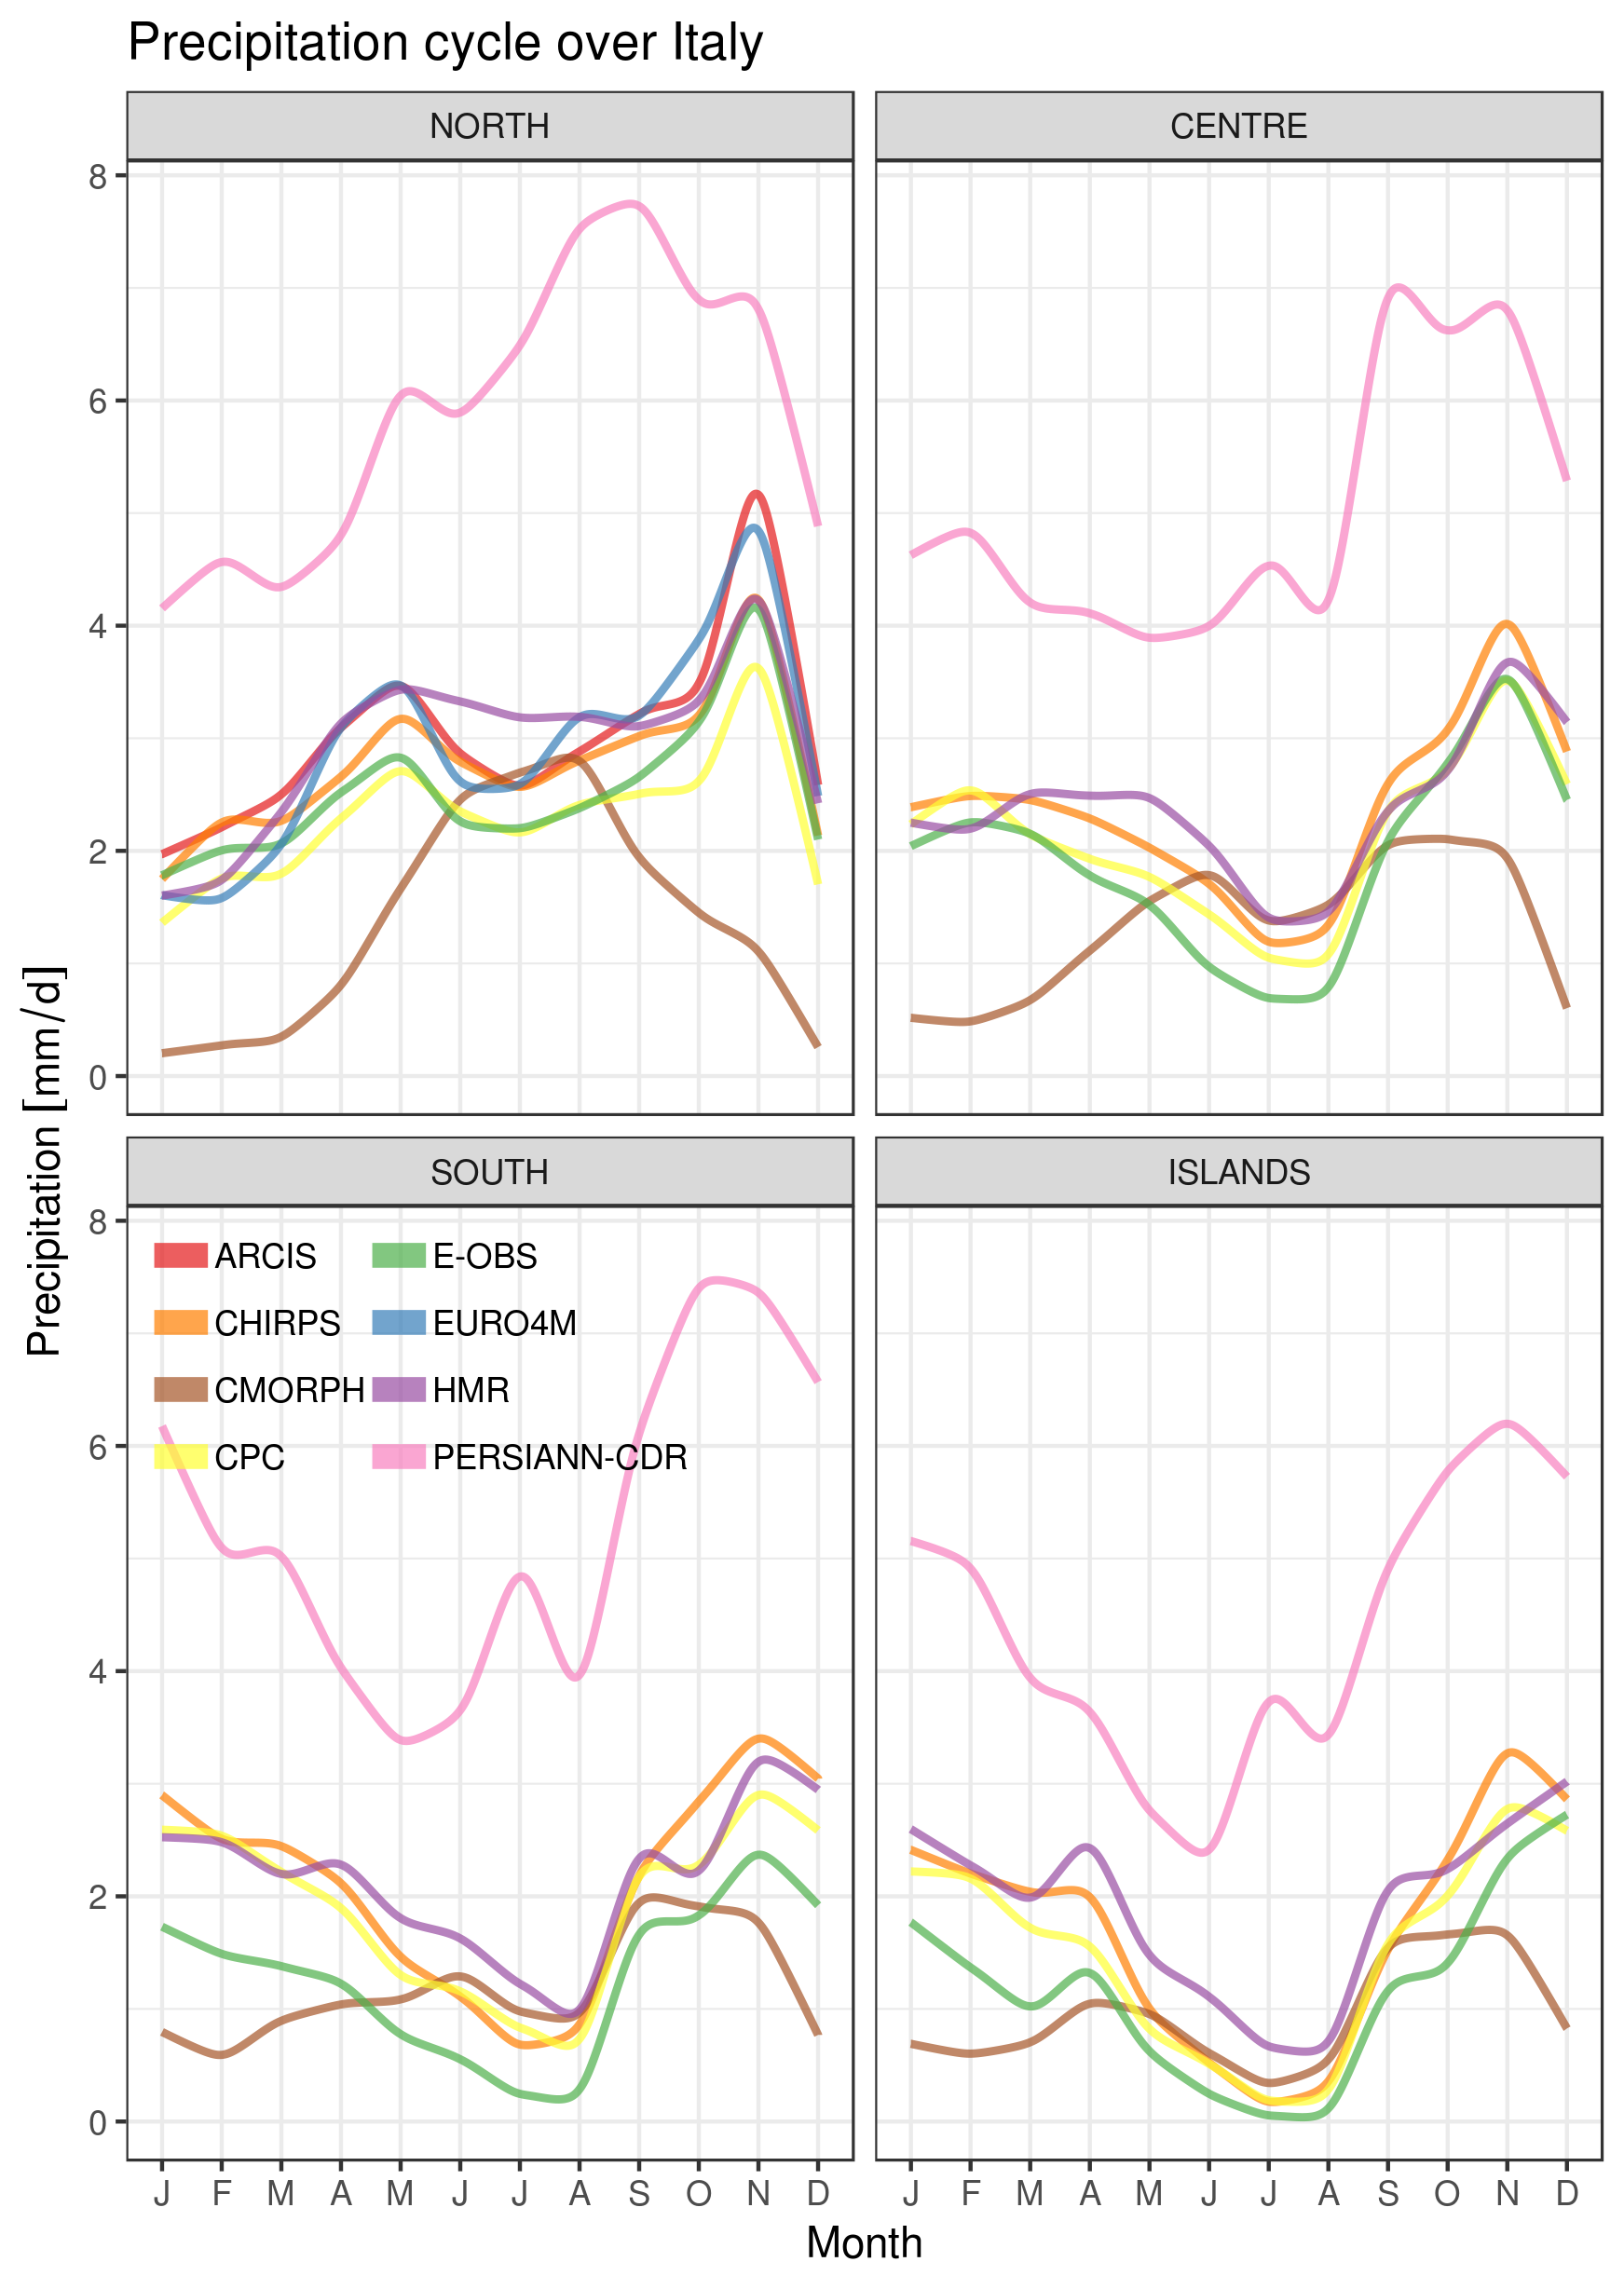
\includegraphics[width=0.7\textwidth]{figures/uncertainty/ac}
    \decoRule
    \caption[Precipitation annual cycle: uncertainty over Italy]{
        Annual cycle for average precipitation for the datasets in \cref{tab:uncertainty_pr}. The four summarising regions are highlighted in \cref{fig:uncertainty_pr_mean,fig:uncertainty_pr_r95,fig:uncertainty_pr_r99}.
} \label{fig:uncertainty_pr_ac}
\end{figure}

The spatial distribution of extreme precipitation can be assessed by \cref{fig:uncertainty_pr_r95,fig:uncertainty_pr_r99}. The three high resolution ARCIS, EURO4M-APGD and HMR datasets capture similar spatial details and amount of extremes in the North, with HMR slightly underestimating. In the other regions, large variability is present: CHIRPS almost completely lacks extremes, while CPC and PERSIANN-CDR show limited spatial variability across the regions. CMORPH, on the other hand, presents spatial patterns that are completely different from those obtained by the other products.\\
The Probability Density Functions of rainy days (\cref{fig:uncertainty_pr_pdf1,fig:uncertainty_pr_pdf2}) confirms the ability of ARCIS and HMR, in the North, to reproduce precipitation extremes not available in the other datasets. In the other regions, no clear picture seems to be discernible from the PDF data, with CHIRPS, CMORPH and HMR generally showing more intense extremes. In the South and in the Islands, E-OBS shows the least amount of extremes, while CMORPH continues to show much stronger seasonal variations compared to the other datasets.
\begin{figure}
    \centering
        \includegraphics[width=0.7\textwidth]{figures/uncertainty/r95ptot}
    \decoRule
    \caption[Precipitation extreme ($\textrm{R95}_{ptot}$): uncertainty over Italy]{
        Extreme $\textrm{R95}_{ptot}$ precipitation for the datasets in \cref{tab:uncertainty_pr}. $\textrm{R95}_{ptot}$ represents the percentage of precipitation due to precipitation events above the 95th percentile.
} \label{fig:uncertainty_pr_r95}
\end{figure}
\begin{figure}
    \centering
        \includegraphics[width=0.7\textwidth]{figures/uncertainty/r99ptot}
    \decoRule
    \caption[Precipitation extreme ($\textrm{R99}_{ptot}$): uncertainty over Italy]{
        As \cref{fig:uncertainty_pr_r95}, but for $\textrm{R99}_{ptot}$.
} \label{fig:uncertainty_pr_r99}
\end{figure}
% \begin{figure}
%     \centering
%     \begin{subfigure}{0.8\textwidth}
% %        \caption{}\label{fig:uncertainty_pr_pdf/a}
%         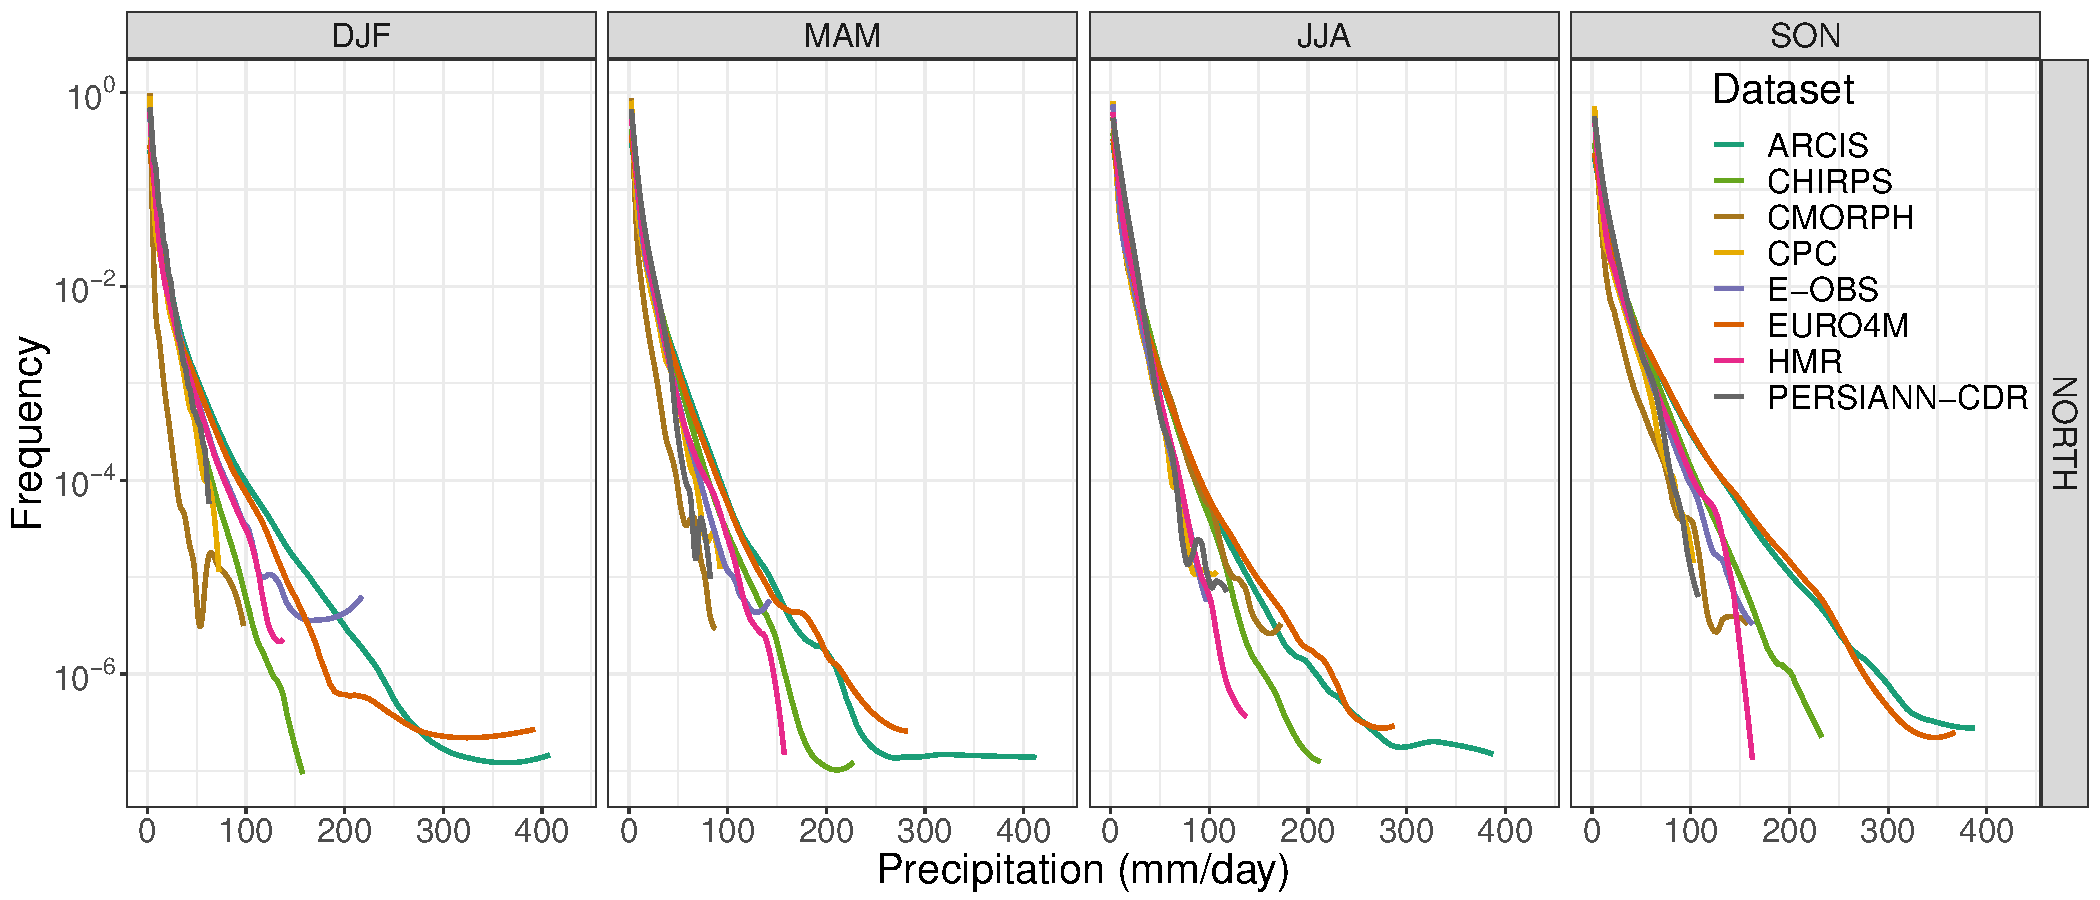
\includegraphics[width=\textwidth]{figures/uncertainty/pdf_NORTH_lines}
%     \end{subfigure}\\
%     \begin{subfigure}{0.8\textwidth}
% %        \caption{}\label{fig:uncertainty_pr_pdf/b}
%         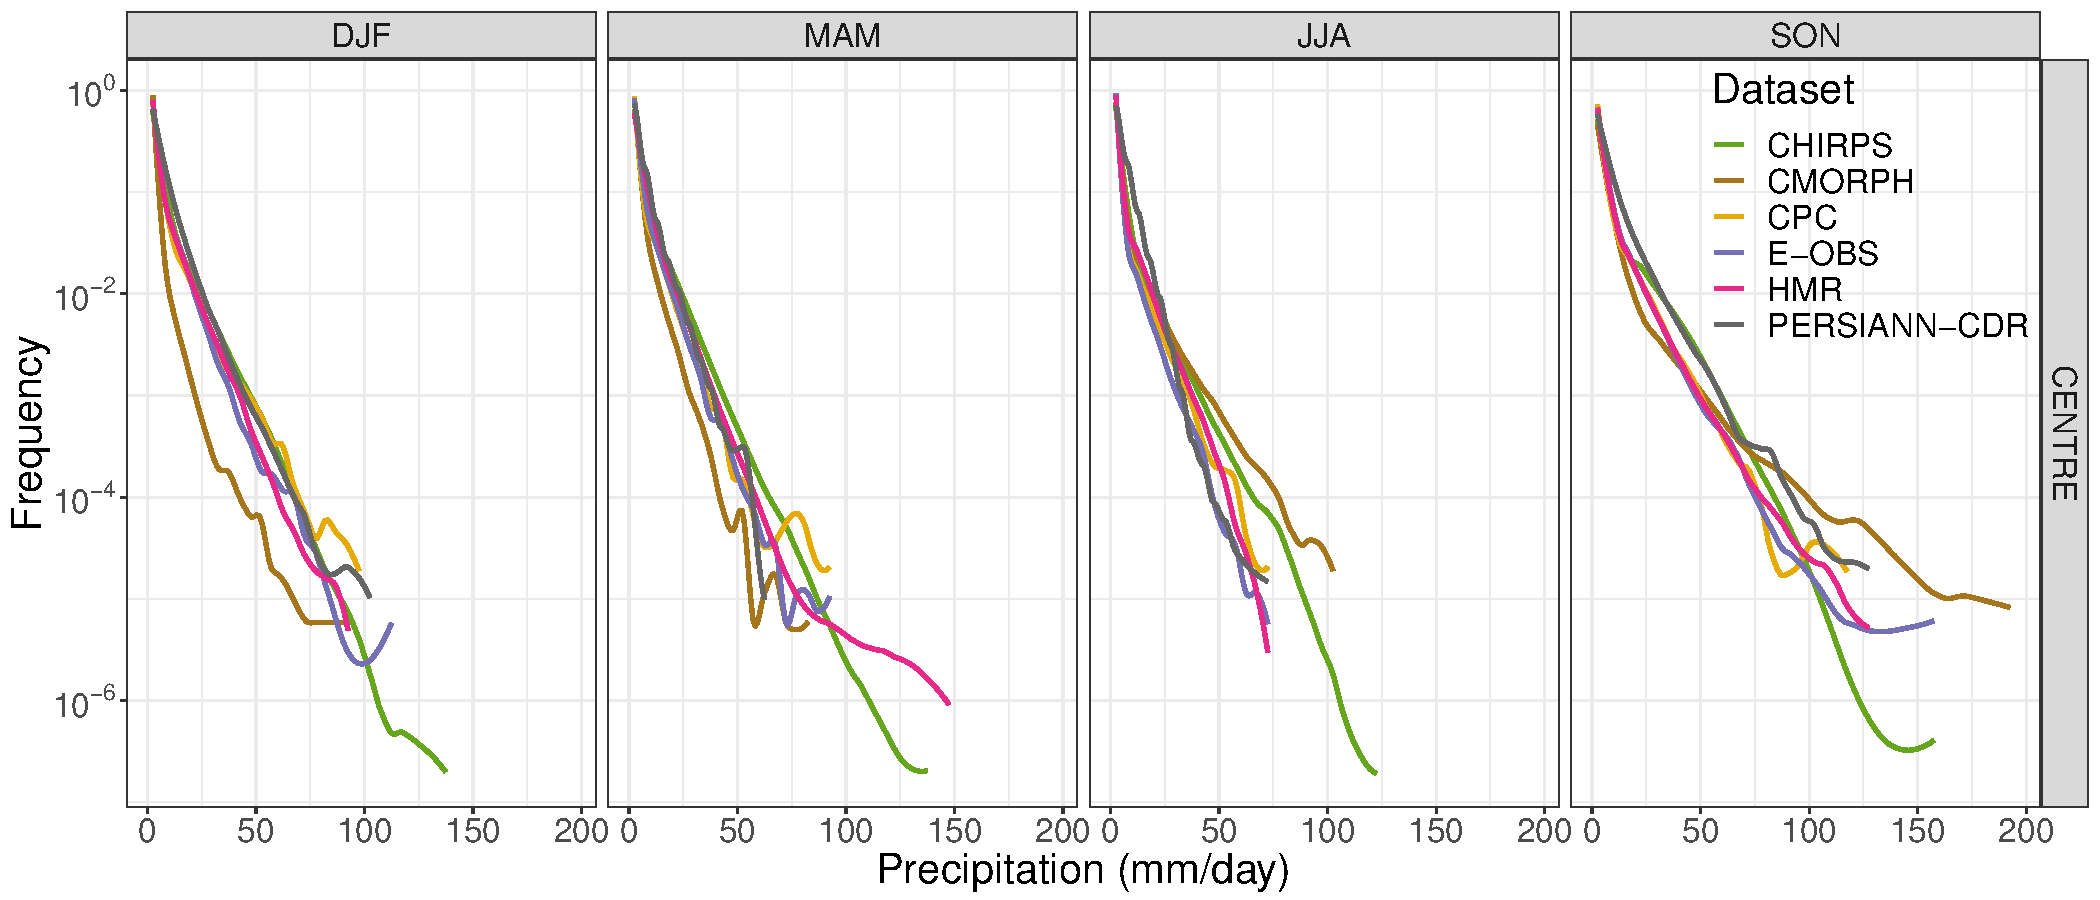
\includegraphics[width=\textwidth]{figures/uncertainty/pdf_CENTRE_lines}
%     \end{subfigure}\\
%     \begin{subfigure}{0.8\textwidth}
% %        \caption{}\label{fig:uncertainty_pr_pdf/c}
%         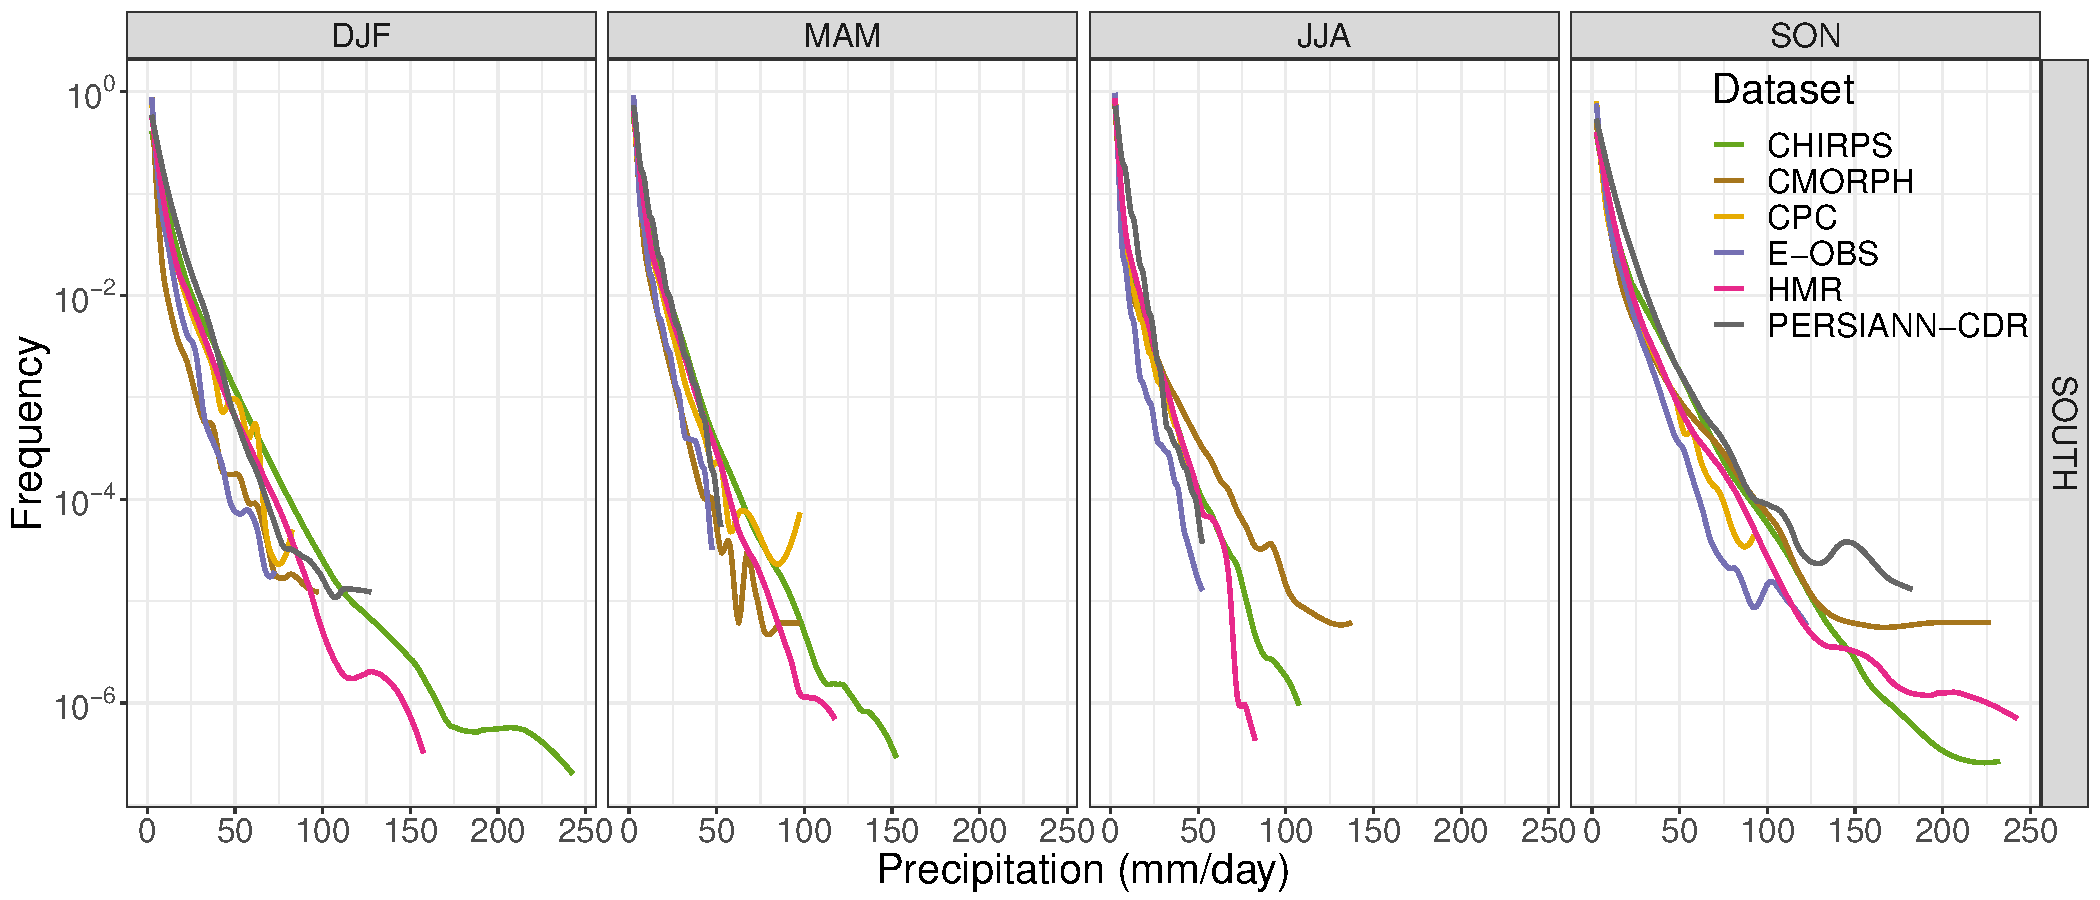
\includegraphics[width=\textwidth]{figures/uncertainty/pdf_SOUTH_lines}
%     \end{subfigure}\\
%     \begin{subfigure}{0.8\textwidth}
% %        \caption{}\label{fig:uncertainty_pr_pdf/d}
%         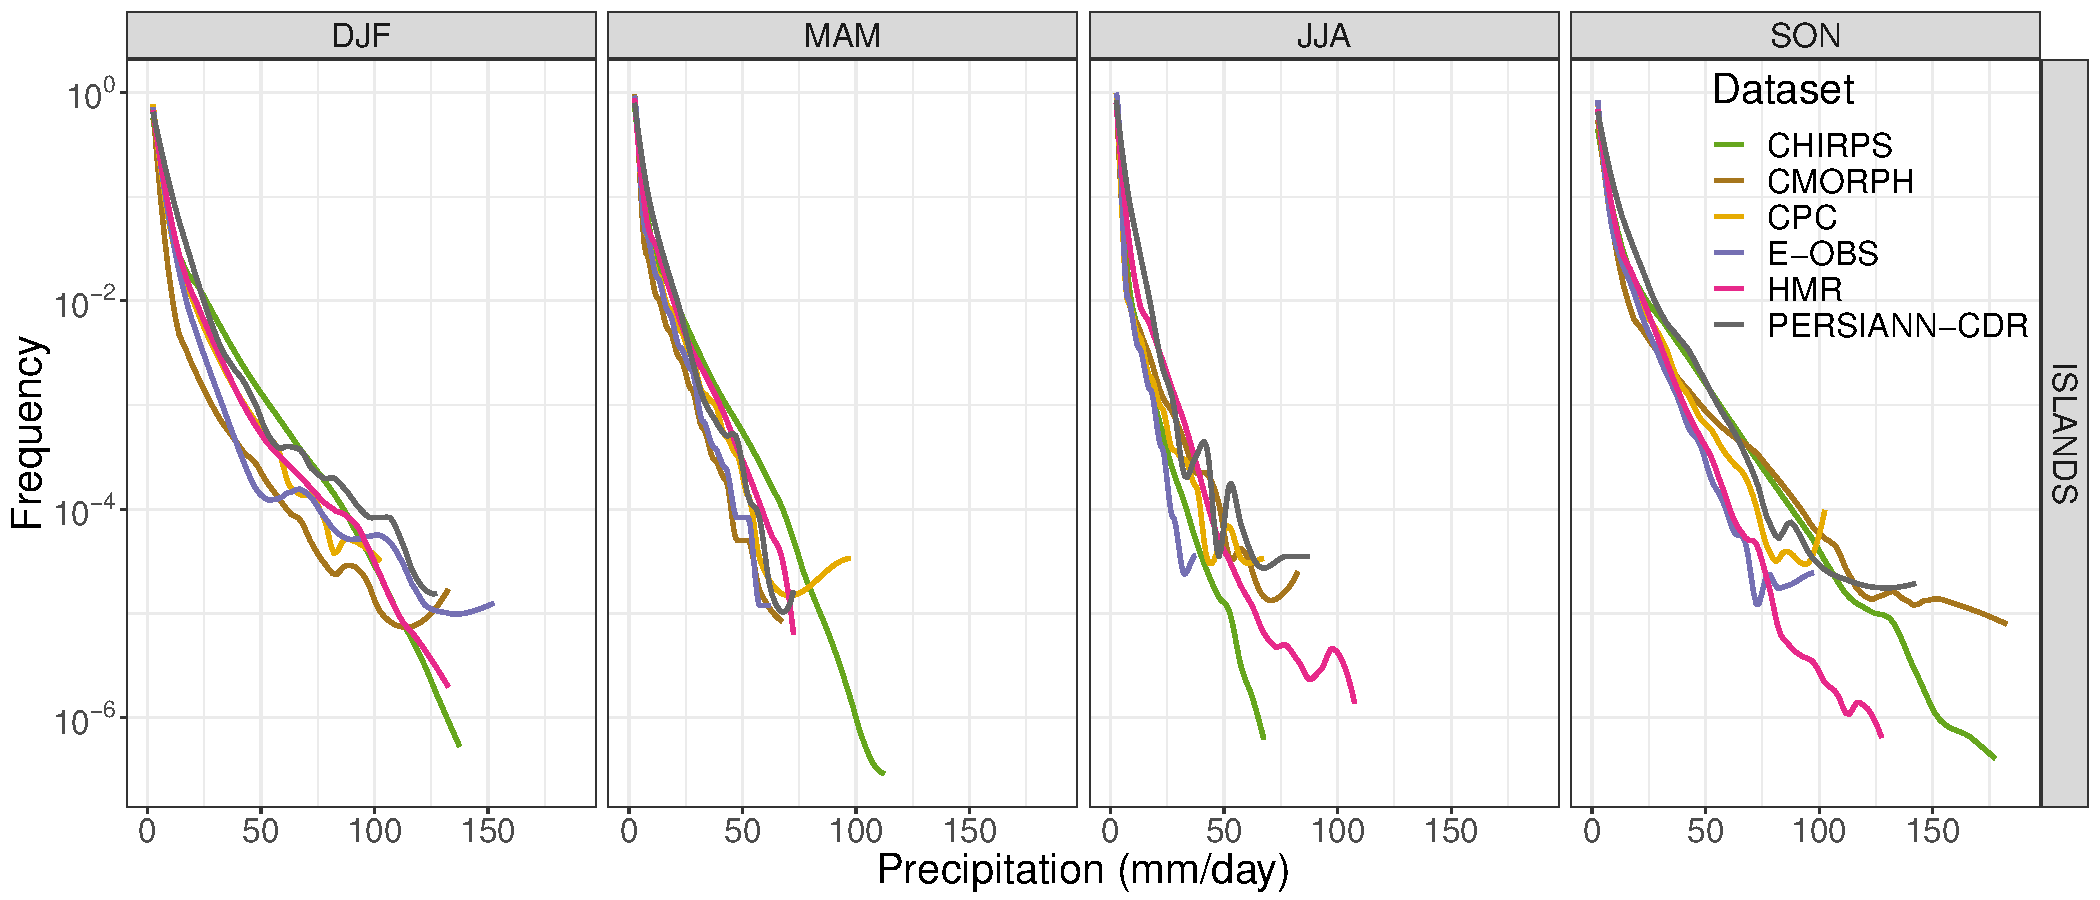
\includegraphics[width=\textwidth]{figures/uncertainty/pdf_ISLANDS_lines}
%     \end{subfigure}
%     \decoRule
%     \caption[Precipitation distribution (PDFs): uncertainty over Italy]{
%         Daily precipitation Probability Density Functions for the datasets in \cref{tab:uncertainty_pr}. The four summarising regions are highlighted in \cref{fig:uncertainty_pr_mean,fig:uncertainty_pr_r95}.
%     }\label{fig:uncertainty_pr_pdf}
% \end{figure}
\begin{sidewaysfigure}
    \centering
        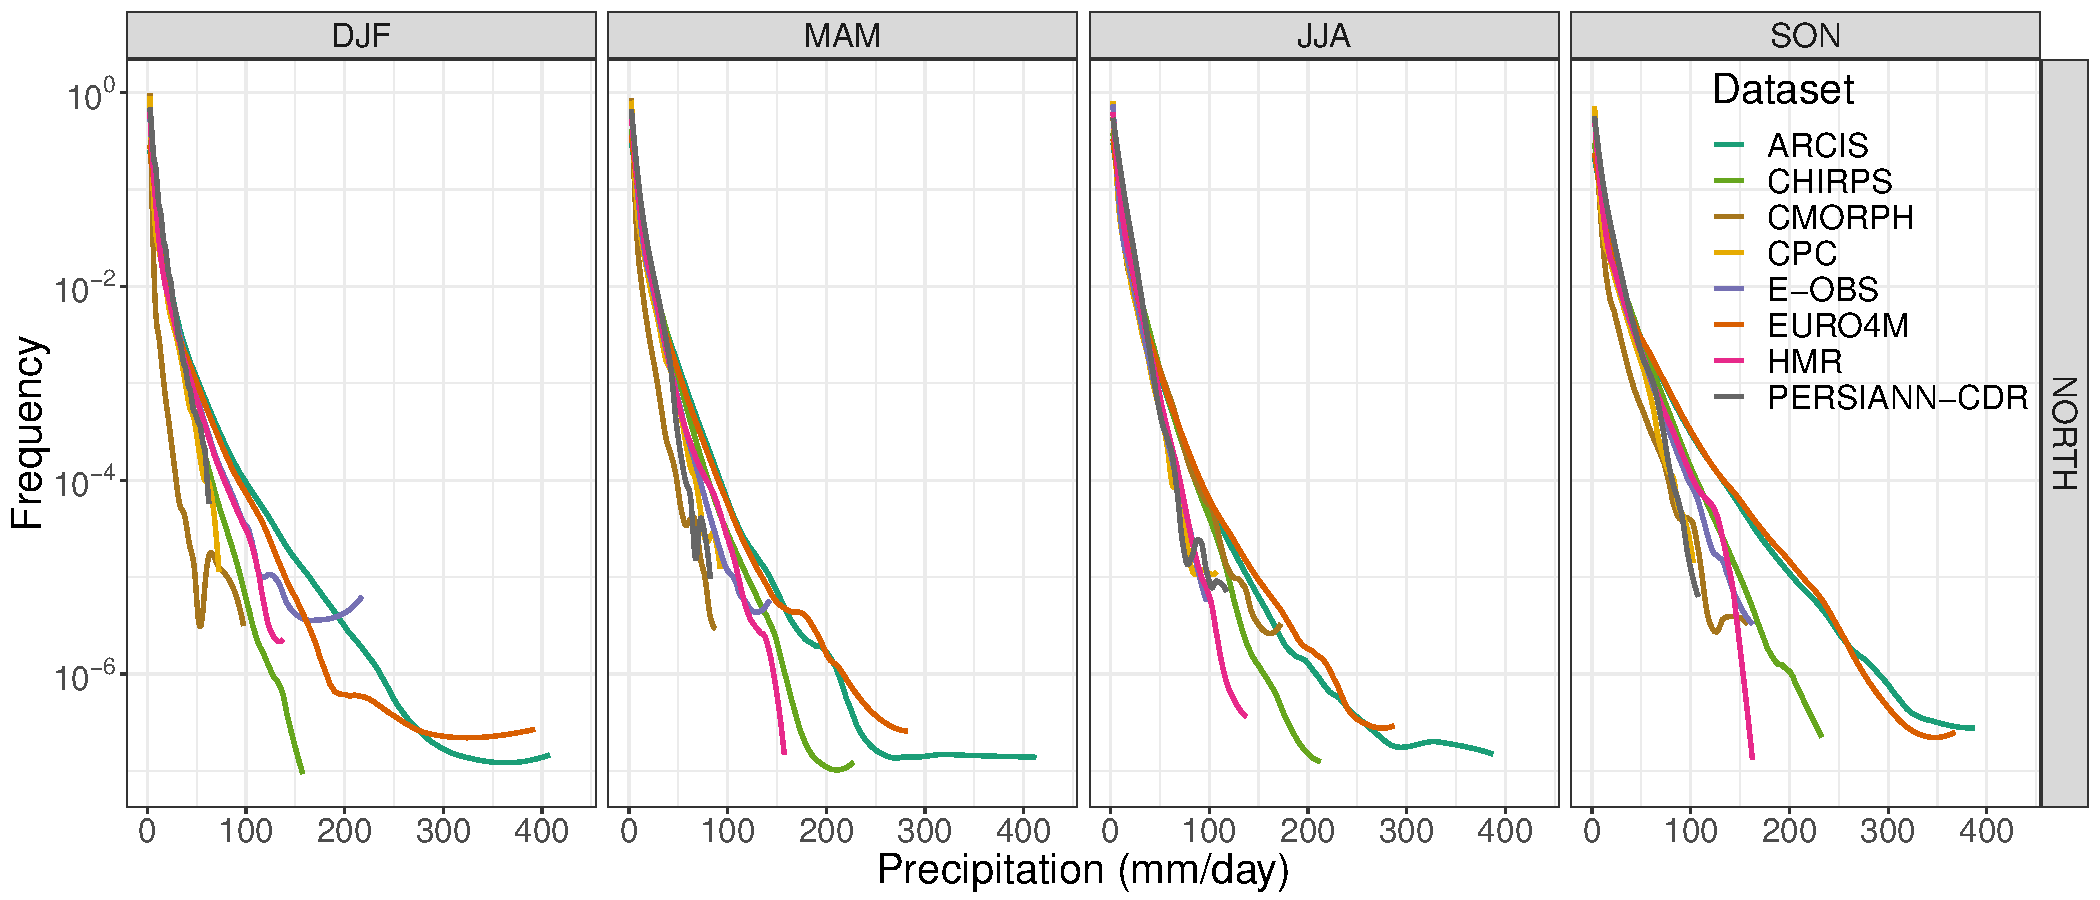
\includegraphics[width=0.8\textheight]{figures/uncertainty/pdf_NORTH_lines}
        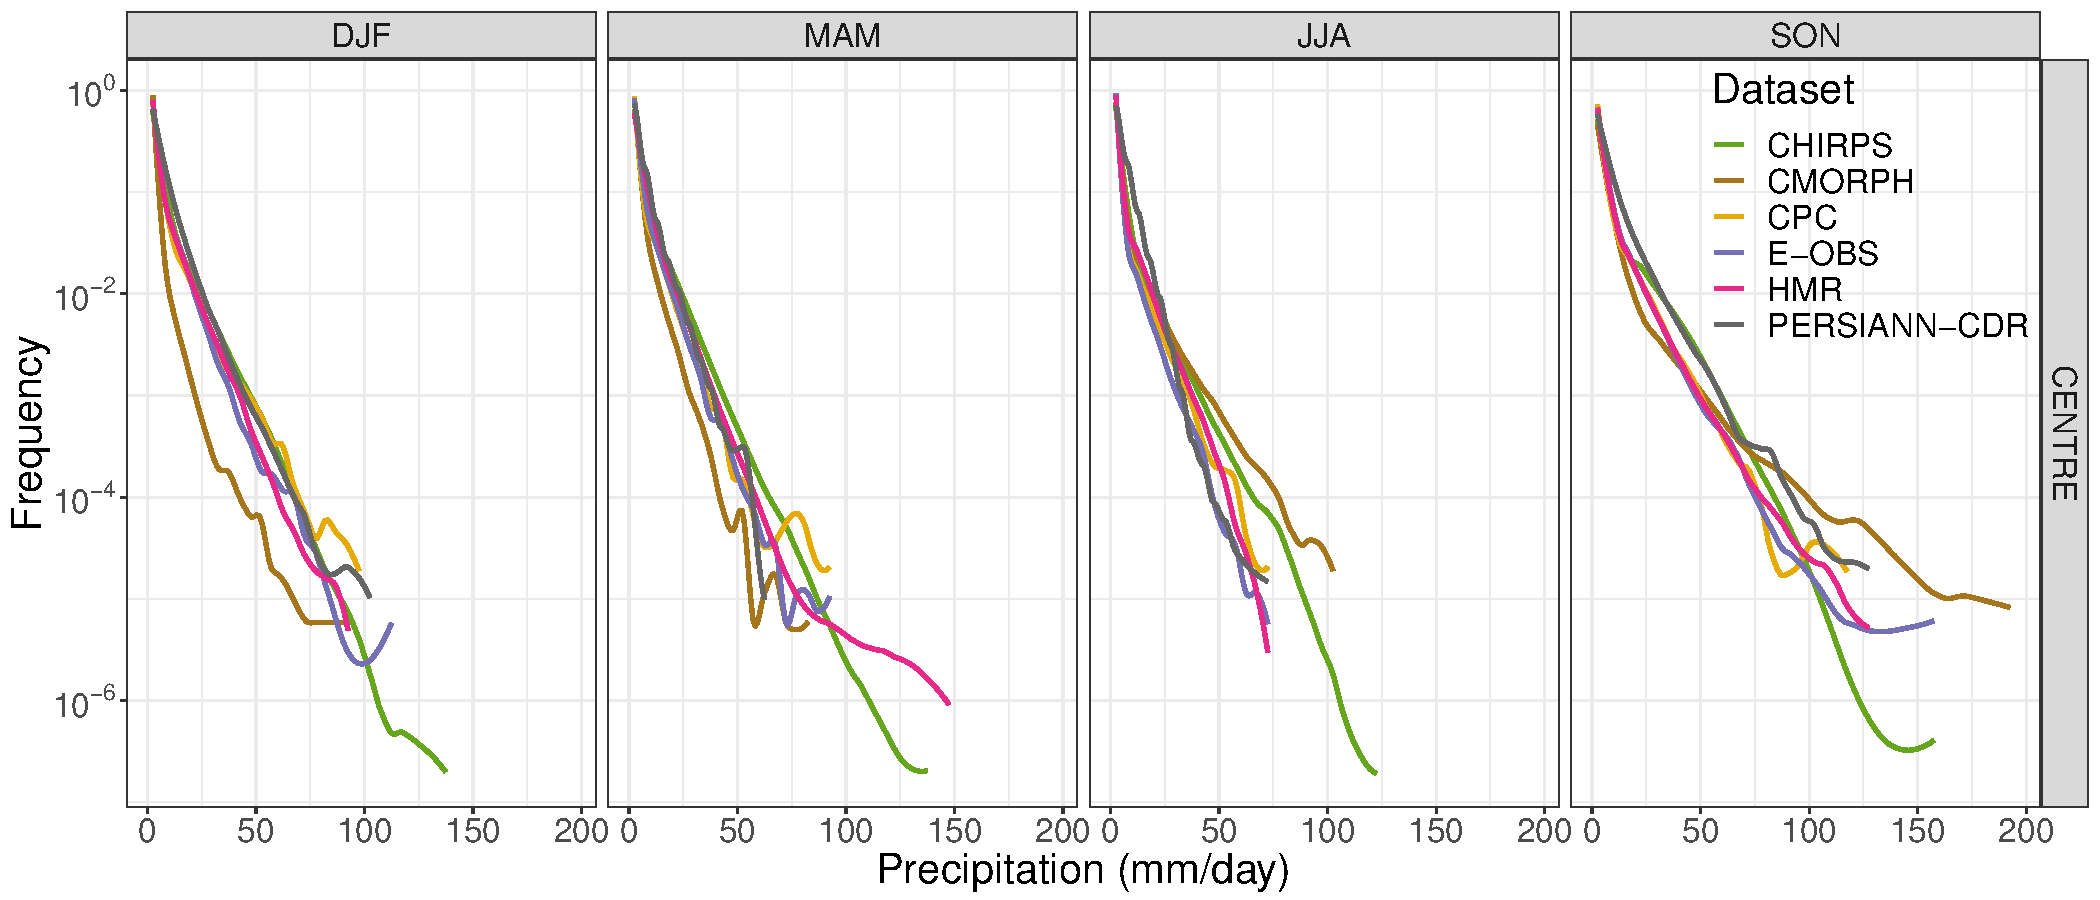
\includegraphics[width=0.8\textheight]{figures/uncertainty/pdf_CENTRE_lines}
    \caption[Precipitation distribution (PDFs): uncertainty over Italy (1)]{
        Daily precipitation Probability Density Functions for the datasets in \cref{tab:uncertainty_pr} for the North and Centre regions. The four summarising regions are highlighted in \cref{fig:uncertainty_pr_mean,fig:uncertainty_pr_r95}.
    }\label{fig:uncertainty_pr_pdf1}
\end{sidewaysfigure}
\begin{sidewaysfigure}
    \centering
        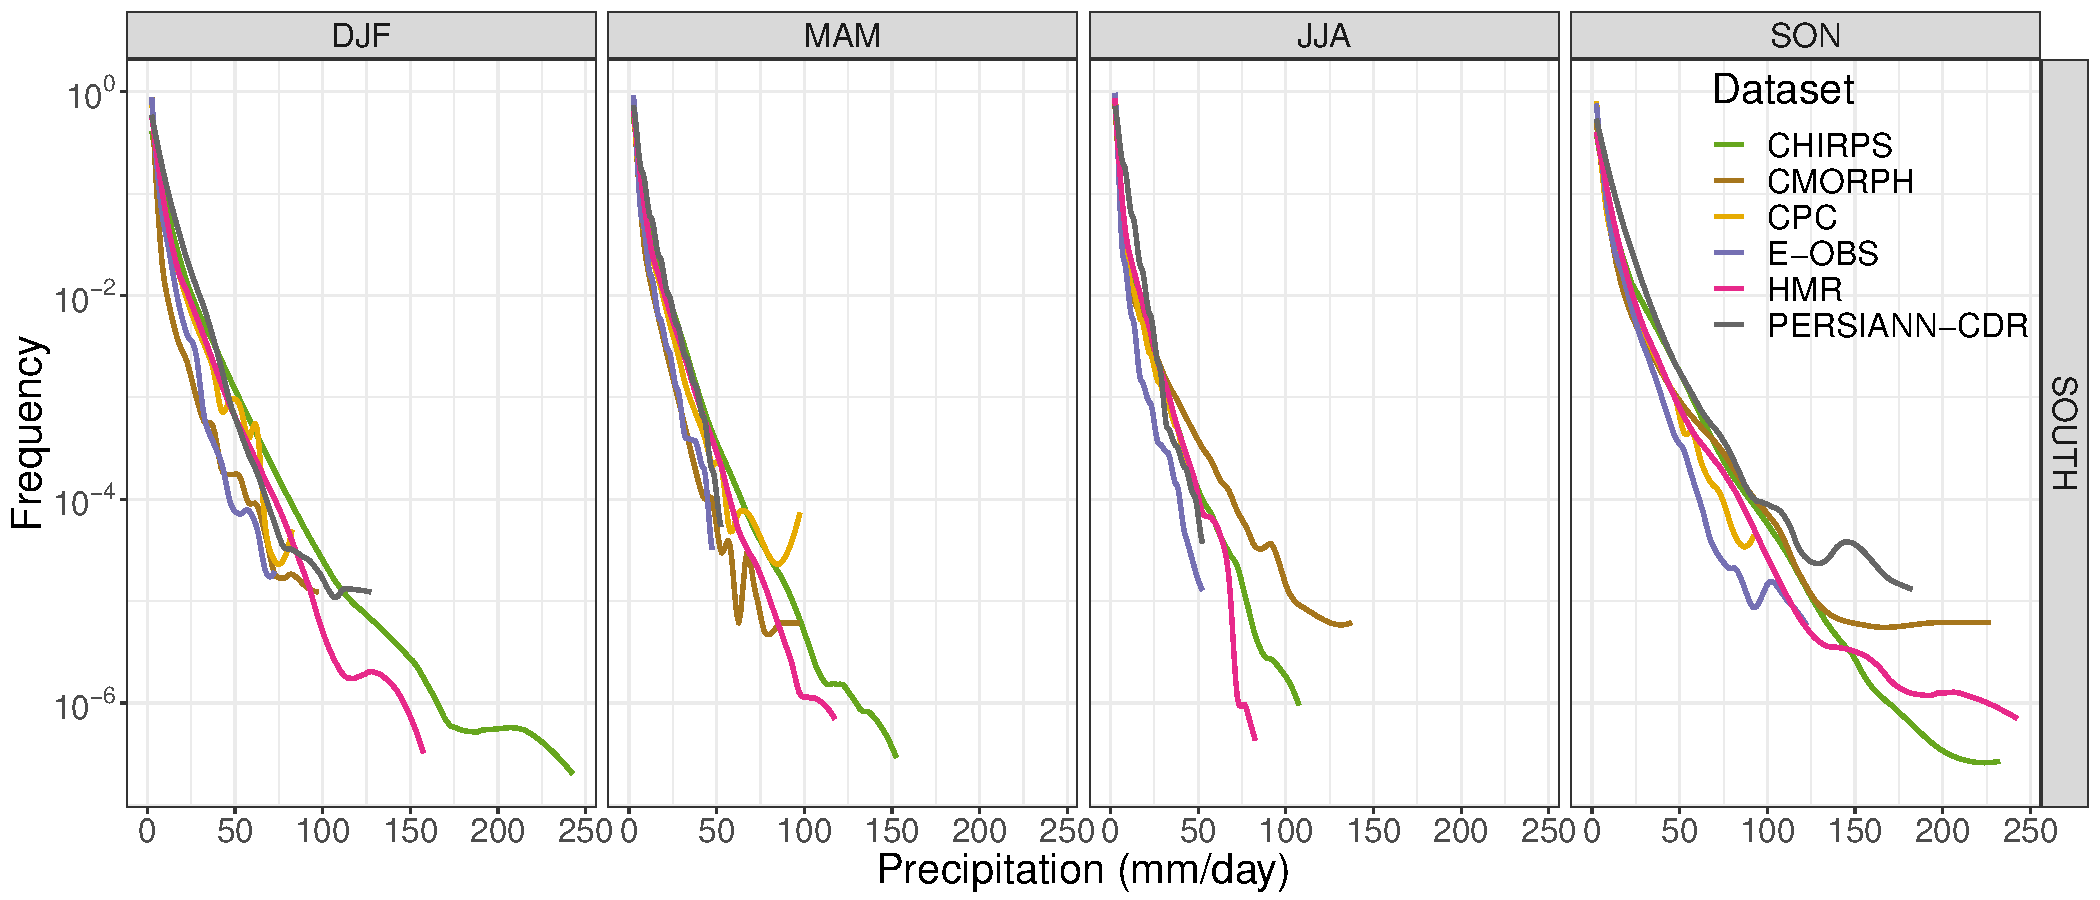
\includegraphics[width=0.8\textheight]{figures/uncertainty/pdf_SOUTH_lines}
        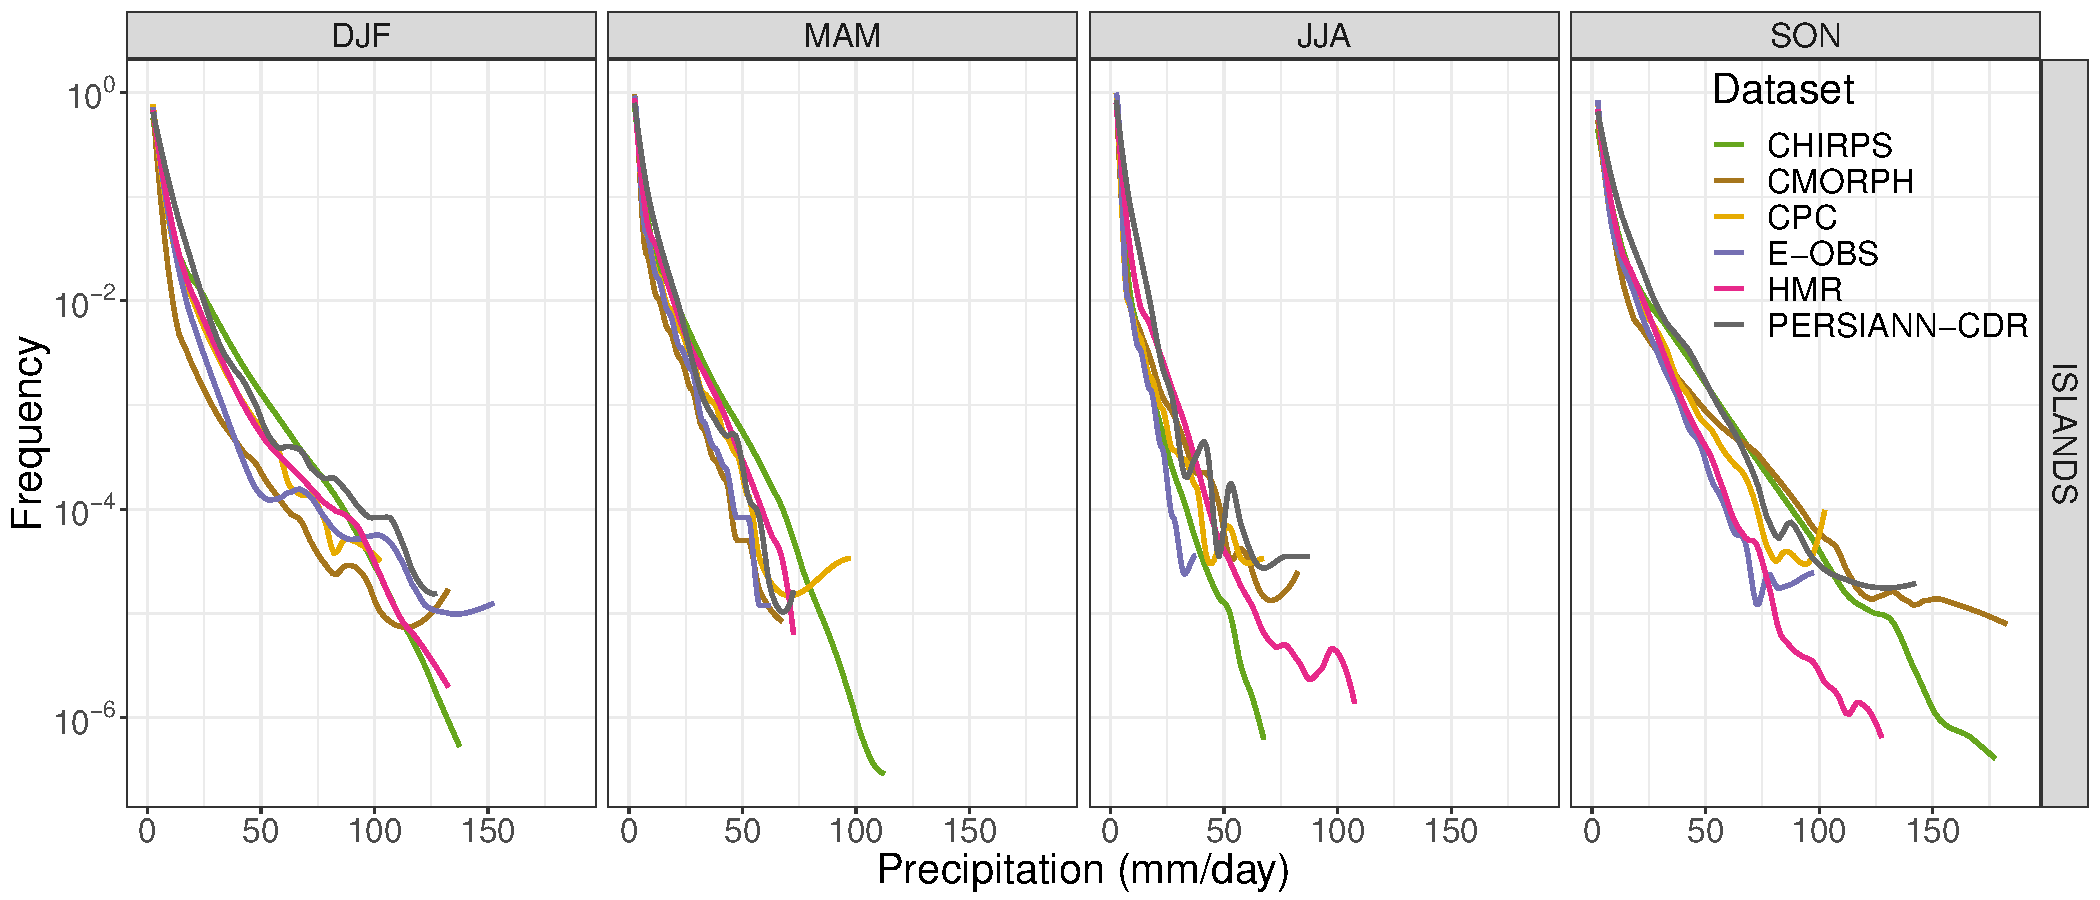
\includegraphics[width=0.8\textheight]{figures/uncertainty/pdf_ISLANDS_lines}
    \decoRule
    \caption[Precipitation distribution (PDFs): uncertainty over Italy (2)]{
        As \cref{fig:uncertainty_pr_pdf1}, but for the South and Islands regions.
    }\label{fig:uncertainty_pr_pdf2}
\end{sidewaysfigure}

These results show that the uncertainty associated with precipitation observations is often large, especially when it comes to precipitation extremes. In this analysis, two of the eight datasets considered (CMORPH and PERSIANN-CDR), both of which solely based on satellite data, showed very large biases (one underestimating, one overestimating) even in average precipitation, indicating that the performance of satellite-based products is insufficient in this specific region. Additionally, gauge undercatch is not taken into consideration in any of the station-based datasets employed in this brief analysis, thus uncertainty, especially for winter extreme events in mountainous regions, might be very large. On the positive side, the two Northern high-resolution datasets (EURO4M-APGD and ARCIS) show good agreement, with the HMR European reanalysis also showing good performance for mean precipitation (but a general underestimation of extremes compared to other datasets).


%------------------------------------
%	DISCHARGE OBS
%------------------------------------
\section{Discharge observations} \label{sec:disch_obs}
River discharge observations are necessary to evaluate the performance of hydrological models.
For a given river location, discharge is calculated from water level observations assuming a given \emph{stage-discharge} (or \emph{rating}) curve \citep{Braca2008}, which takes into account riverbed shape and water speed.
Stage-discharge curves are extensively used in hydrology, but they necessitate constant updates due to the fact that stream channels constantly change due to erosion, deposition of debris, vegetation growth and presence of ice.
As a consequence, despite being an irreplaceable tool, discharge measurements can sometimes be somewhat unreliable, especially for high flows \citep{DiBaldassarre2009}.\\ 
In this thesis work, datasets of discharge from several sources are considered. Similarly to the precipitation dataset exposed in \cref{chp:itaobs}, three hourly discharge datasets were provided by Prof. Marco Verdecchia\footnote{\url{http://www.dsfc.univaq.it/it/ricercatori/44-verdecchia-marco.html}}, from the University of L'Aquila; to these, the standard European Water Archive \citep{EWA2014}, containing daily data from a collection of sources over Europe, was added.
Due to the low number of daily discharge stations over Italy (only three according to the official reference\footnote{\url{ftp://ftp.bafg.de/pub/REFERATE/GRDC/website/grdc_referencestations_summary_countries.pdf}}), the Global Runoff Data Centre (GRDC) database was not selected for use in this study.
\begin{figure}
    \centering
    % source of this data if you want to remake it:
    % /home/afantini/places/clima-archive/flood/discharge_stations/dst_merge/
    \begin{subfigure}{.475\textwidth}
%        \caption{}\label{fig:disch_dst/a}
        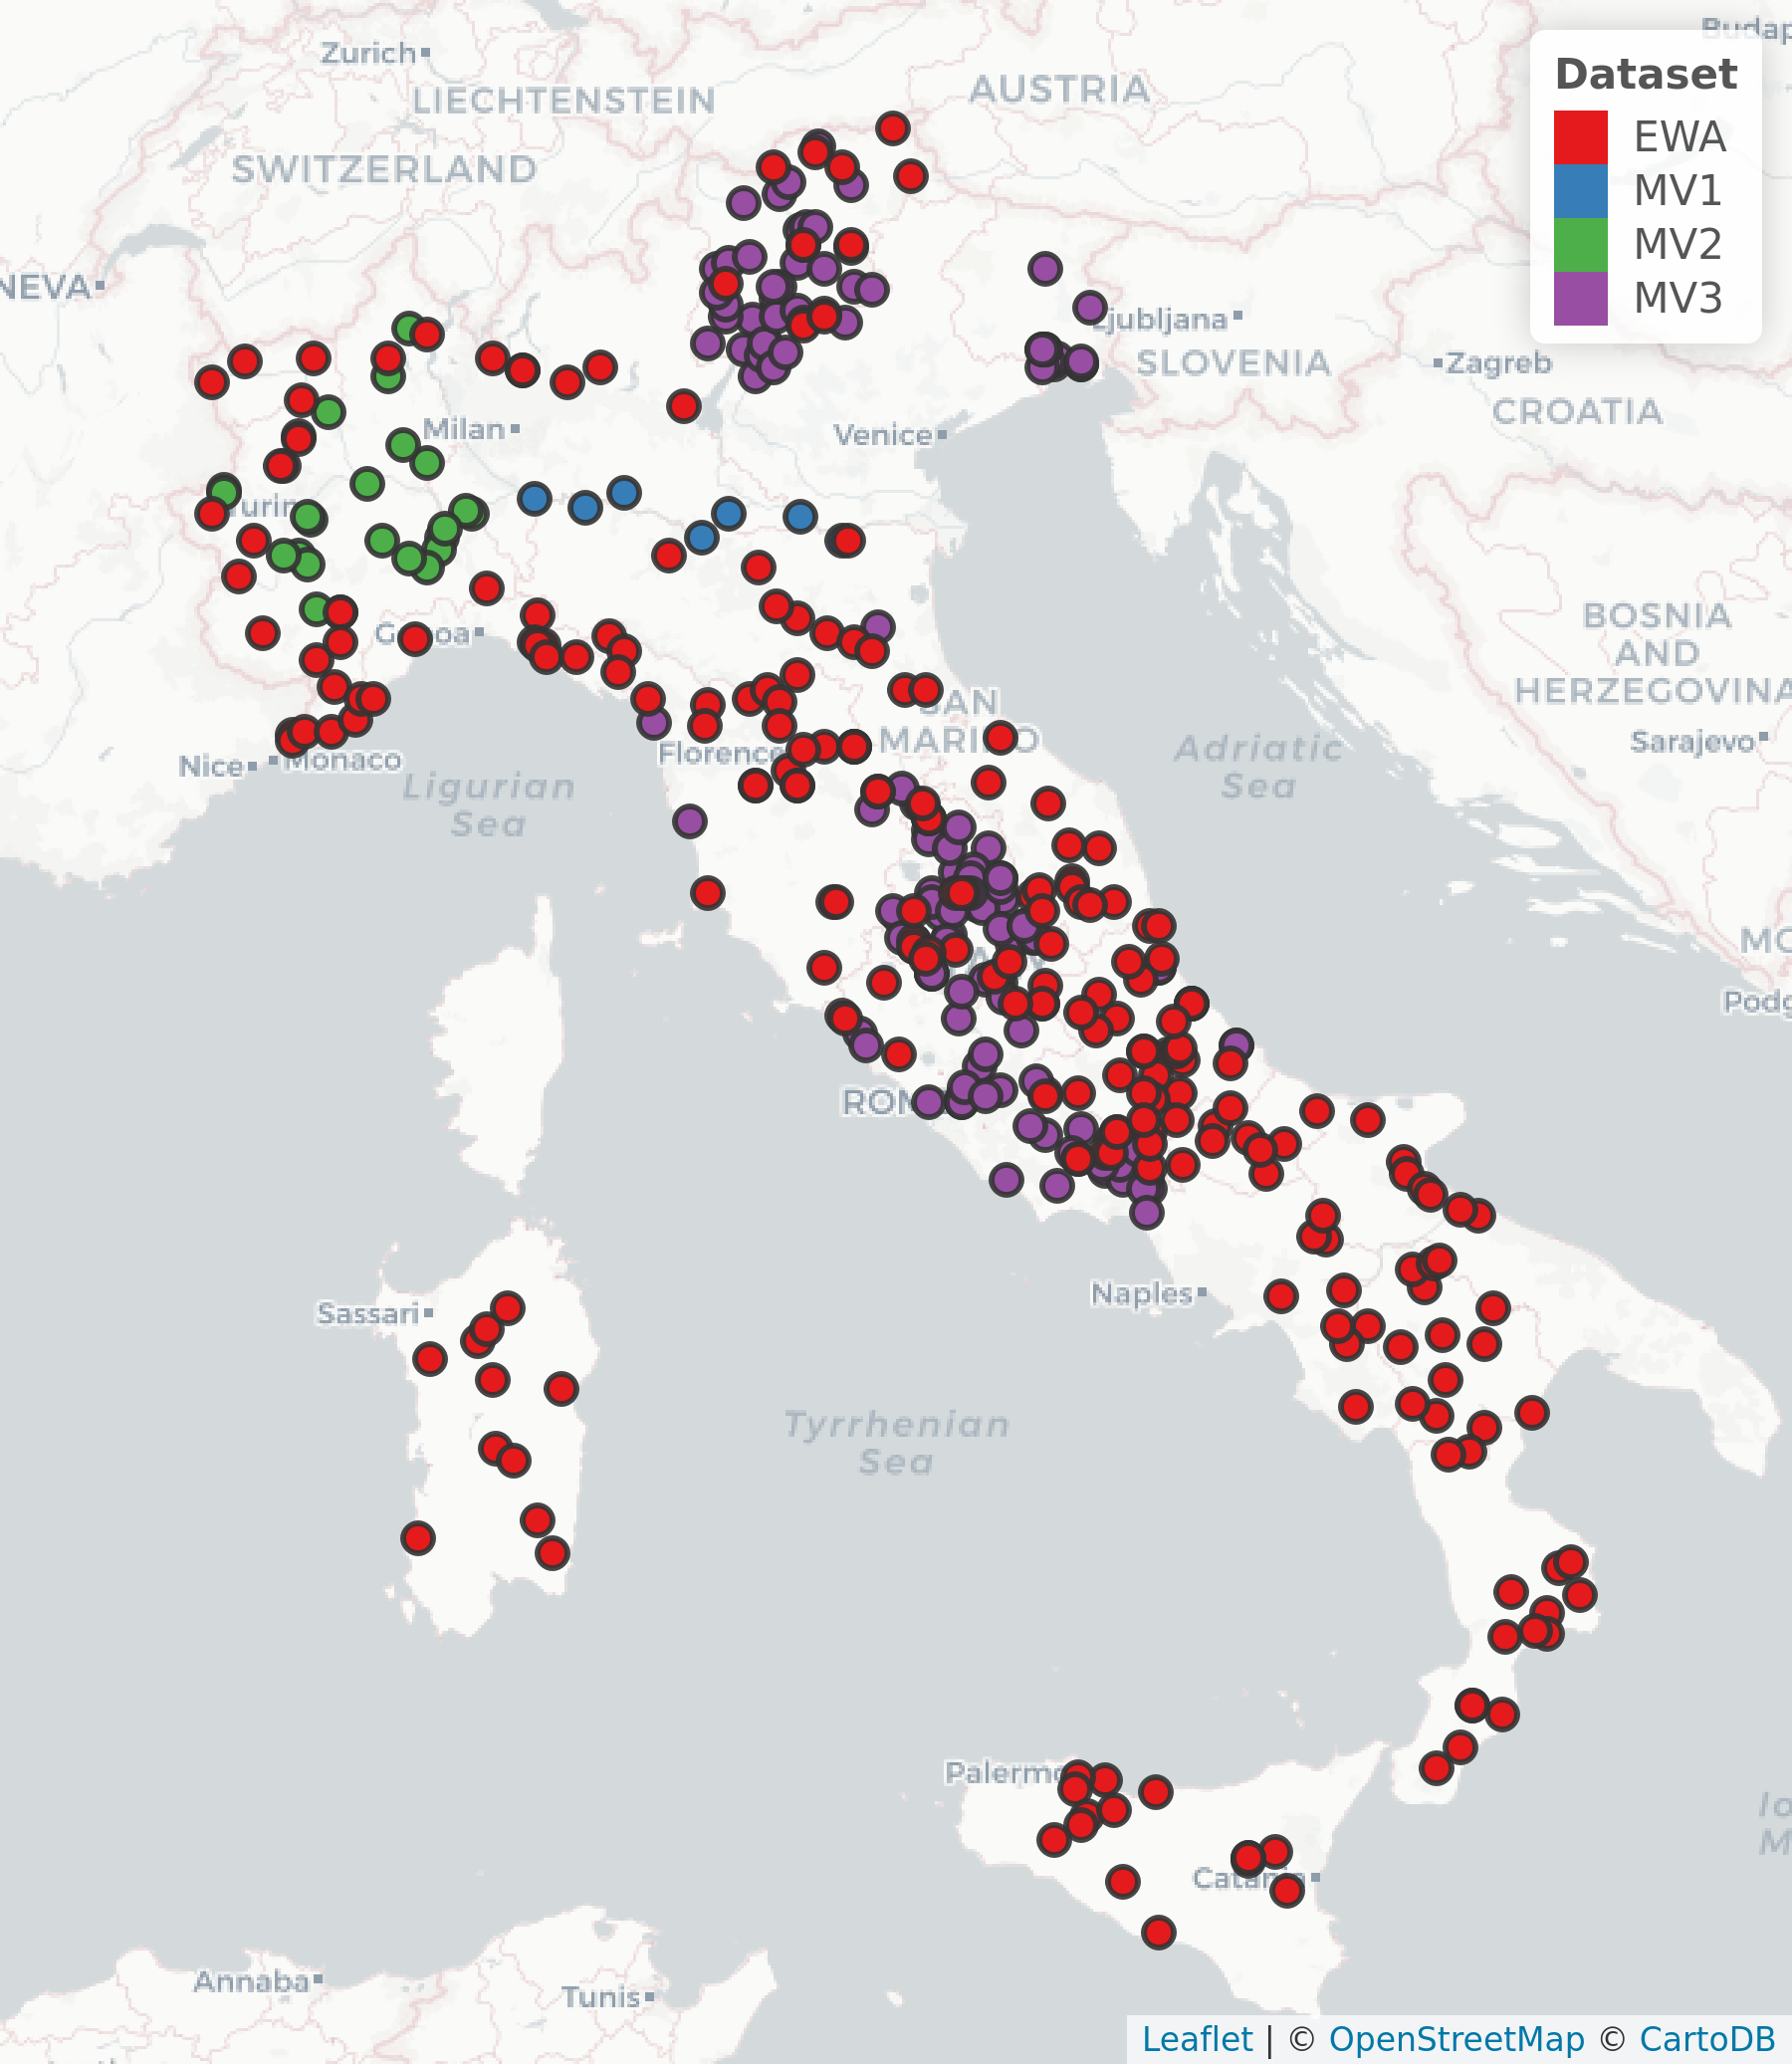
\includegraphics[width=\textwidth]{figures/allstats_ita}
    \end{subfigure}
    \begin{subfigure}{.475\textwidth}
%        \caption{}\label{fig:disch_dst/b}
        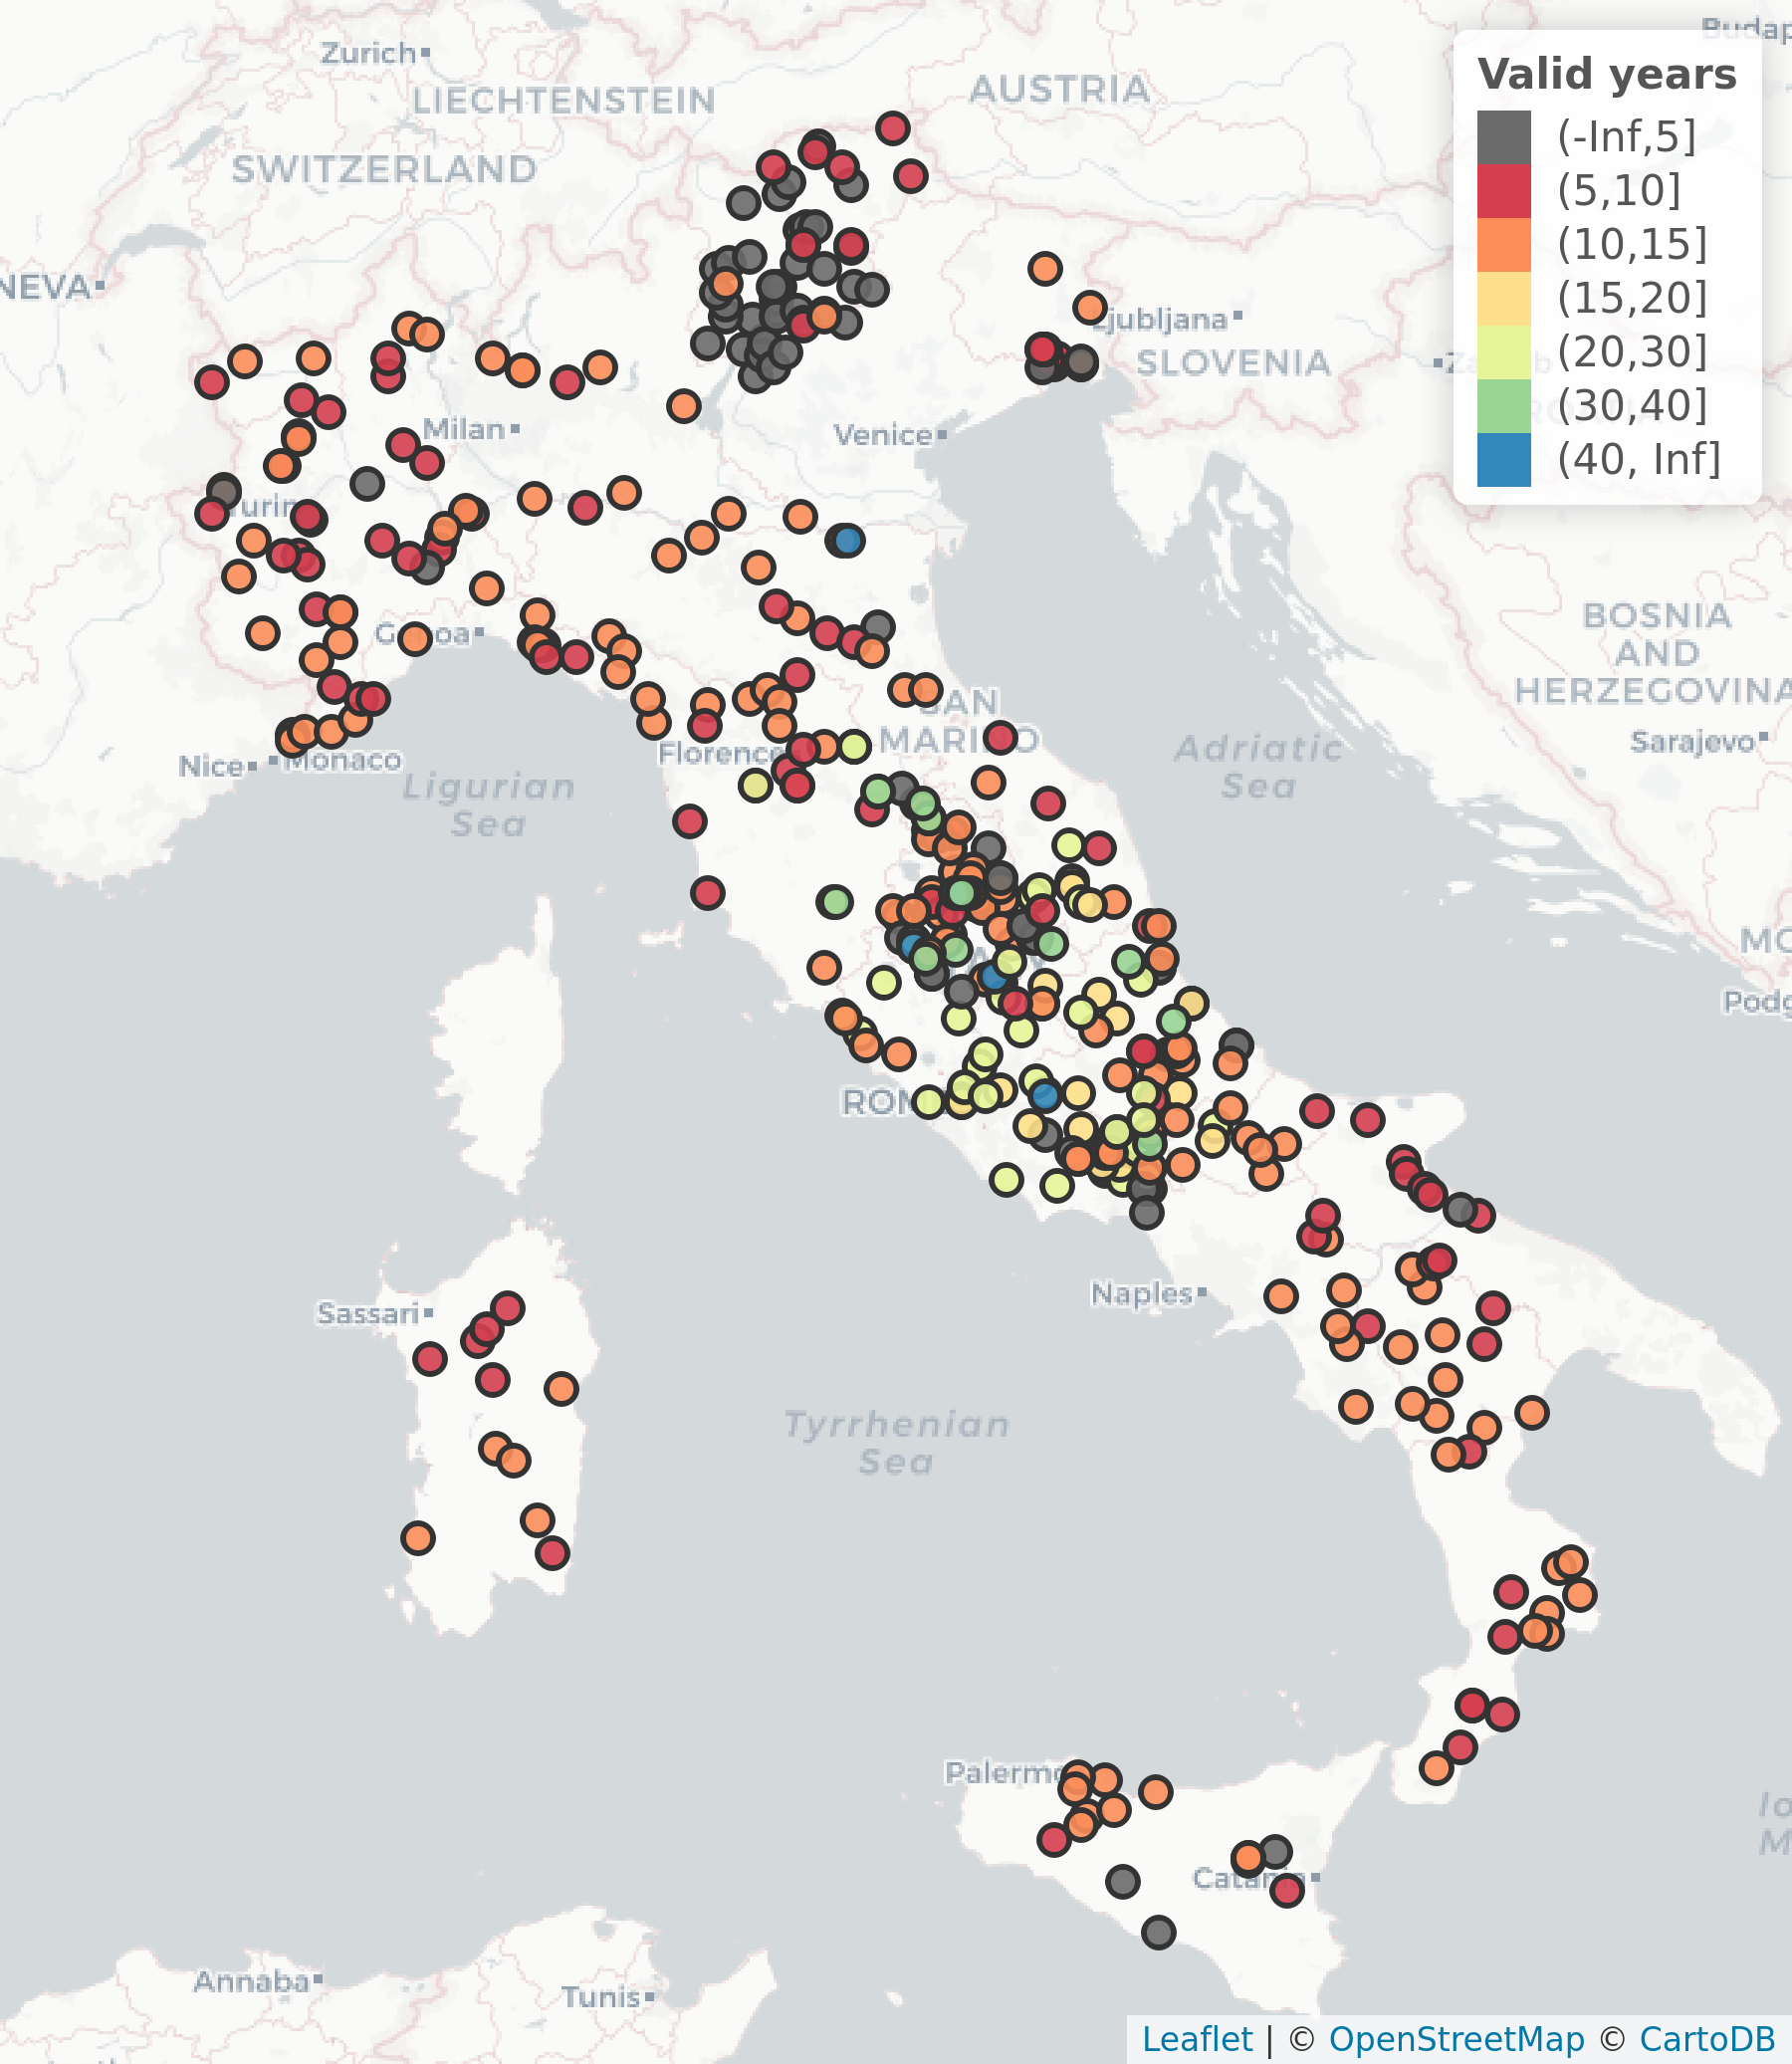
\includegraphics[width=\textwidth]{figures/allstats_ita_2}
    \end{subfigure}
    \decoRule
    \caption[Location and time availability of the 414 discharge stations considered]{Source dataset (left) and time availability (right, in years) of the 414 discharge stations over the Italian territory, from the four datasets of \cref{tab:disc_dst}.} \label{fig:disch_dst}
\end{figure}

\Cref{tab:disc_dst} shows information about the four available datasets, while \cref{fig:disch_dst} shows the number of valid data years over Italy for each station, prior to any data checking.
The coverage of the Italian territory is not complete, with two regions (Veneto and Puglia) being completely devoid of stations, and other areas (e.g. Trentino--Alto Adige) where temporal station coverage is low, often less than five years. Some stations even have no valid data at all.
Station density and time availability are highest in Central Italy.\\
It has to be stressed that, in many cases, station locations were found to be erroneous (especially for the EWA dataset in Southern Italy); additionally, the time range with available observations varies wildly not only from dataset to dataset, but also within the same dataset.
Data quality problems, ranging from stuck sensors (see e.g. \cref{fig:stuck_disc_sensor}) to extreme outliers, are present in all datasets.\\
For these reasons, when performing data analysis and validation, care has to be taken to select only stations that have a sufficiently long time range, without any noticeable systematic error. To this end, manual controls using several metrics (among which interquartile range, standard deviation to mean ratio, frequency of most common values, number of outliers) and comparison of nearby timeseries are carried out. However, only the most conspicuous errors are guaranteed to be removed by this procedure, and many inhomogeneities and suspicious timeseries remain in the datasets.\\
Similarly to all the other data sources used in this thesis, the four discharge datasets are converted to netCDF files compliant with the CF-1.7 conventions; for additional information on the rationale and the practical advantages of using of this file format, refer to \cref{sec:netcdf}.\\

\begin{figure}
    \centering
        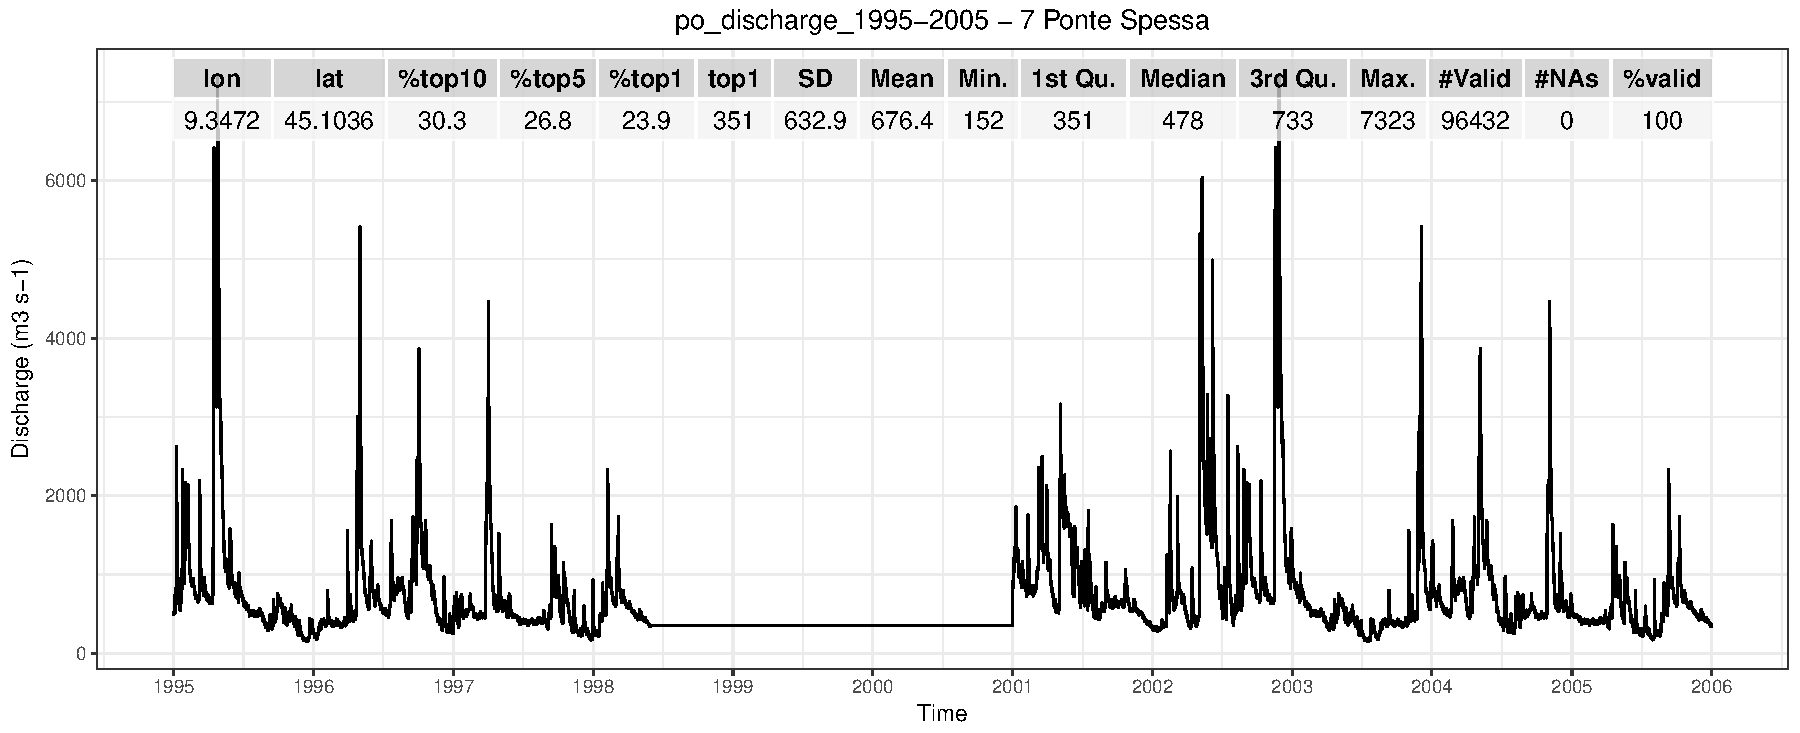
\includegraphics[width=\textwidth]{figures/stuck_discahrge_ts}
    \decoRule
    \caption[Example of a discharge station with a stuck sensor]{
    Example of a discharge station with a sensor stuck at \SI{351}{\cubic\metre\per\second} for almost 3 years. Some station statistics used to assess station quality are listed at the top of the figure.
} \label{fig:stuck_disc_sensor}
\end{figure}

\begin{table}[]
\centering
\begin{tabular}{@{}m{1.3cm}m{1.5cm}m{1.8cm}m{2cm}m{1.8cm}m{1.8cm}@{}}
\toprule
Dataset name & Region & Number of stations & Max period & Frequency & File type \\ \midrule
MV1 & Po river & 7 & 1995--2005 & Hourly & Fortran binary \\
MV2 & Upper Po basin & 43 & 2000--2010 & Hourly & Fortran binary \\
MV3 & Italy & 152 & 2000--2016 & Hourly & Fortran binary \\
EWA & Europe & 4058 (231 in Italy) & 1863--2013 & Daily and monthly & Plain text \\ \bottomrule
\end{tabular}
\caption[List of discharge observations]{Discharge datasets used in this thesis. See \cref{fig:disch_dst} for station locations in Italy. Datasets provided by Marco Verdecchia are named MV1 to MV3.}\label{tab:disc_dst}
\end{table}


%------------------------------------
%	FLOOD OBS
%------------------------------------
\section{Flood extent observations} \label{sec:flood_obs}
Flood extent observations are useful to validate and evaluate model performance against real world flood events.
Unfortunately, availability of precise maps of flooded areas over Italy is lacking due to the aforementioned fragmentation of regional environment agencies and lack of national coordination.
In the last decades, thanks to advancements in flood mapping techniques from satellite, by analysing Landsat, MODIS, Sentinel-1, SRTM and other remotely-retrieved data, several projects have started offering flood monitoring and maps with global or regional extent \citep[see e.g.][]{Clement2017, Schlaffer2015, Martinis2015, SMITH1997, Martinis2013, Brakenridge2003, Westerhoff2013}.\\
The Dartmouth Flood Observatory \citep[DFO,][]{G.R.Brakenridge2015}, for example, provides metadata for all major events worldwide from 1985 to present, including shapefiles indicating affected areas.
These are, however, extremely approximate and do not help in the precise identification of flooded areas (see \cref{fig:DFO_floods_ita}); additionally, only 37 events are reported in Italy in the period 1985--present, in comparison with several hundred events listed by IRPI for the period 1967--present (\cref{fig:flood_events_ita}).
\begin{figure}
    \centering
    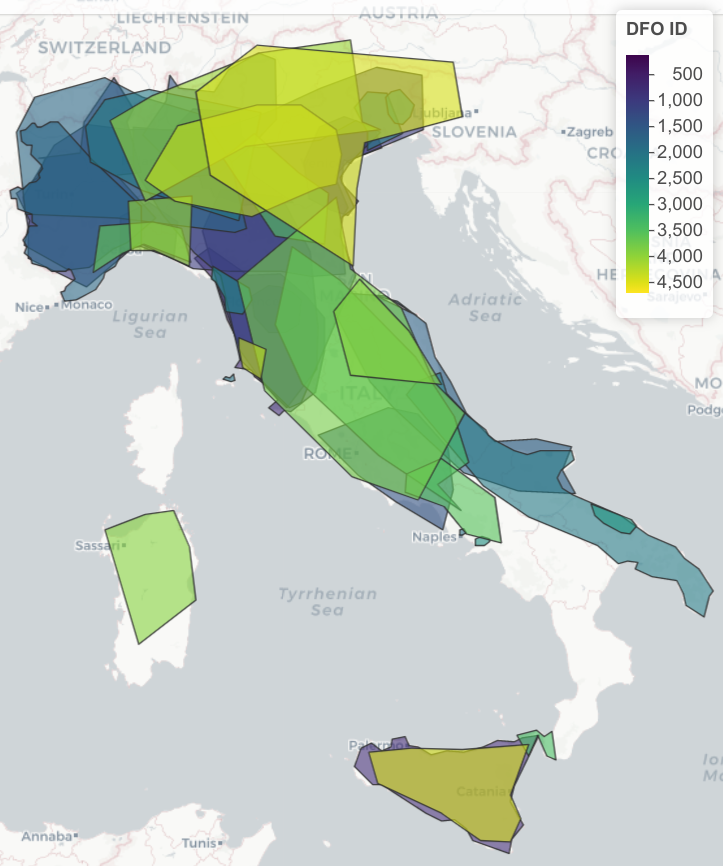
\includegraphics[width=0.7\textwidth]{figures/ita_flood/DFO_floods_ita}
    \decoRule
    \caption[Flooded areas in the DFO database]{
        All areas in Italy affected by a flood event, as provided by the Dartmouth Flood Observatory (DFO). Areas are coloured by their DFO ID.
} \label{fig:DFO_floods_ita}
\end{figure}

The DFO also provides in-depth analysis for specific large events via the NASA-supported Global Flood Monitoring System (GFMS). \Cref{fig:DFO_flood_nov18}, for example, shows the November 2018 flooding in Northern Italy as detected by the DFO algorithms from satellite data: comparing with reported flooding by news sources, only a small part of the flooded areas in Northern Veneto and Liguria is included, and the Sicily flash flooding that caused 9 casualties is not reported at all. For comparison, the NASA NRT Global Flood Mission \citep{Nigro2014} shows even less flooding for the same period and area (\cref{fig:NRT_flood_nov18}).
\begin{figure}
    \centering
    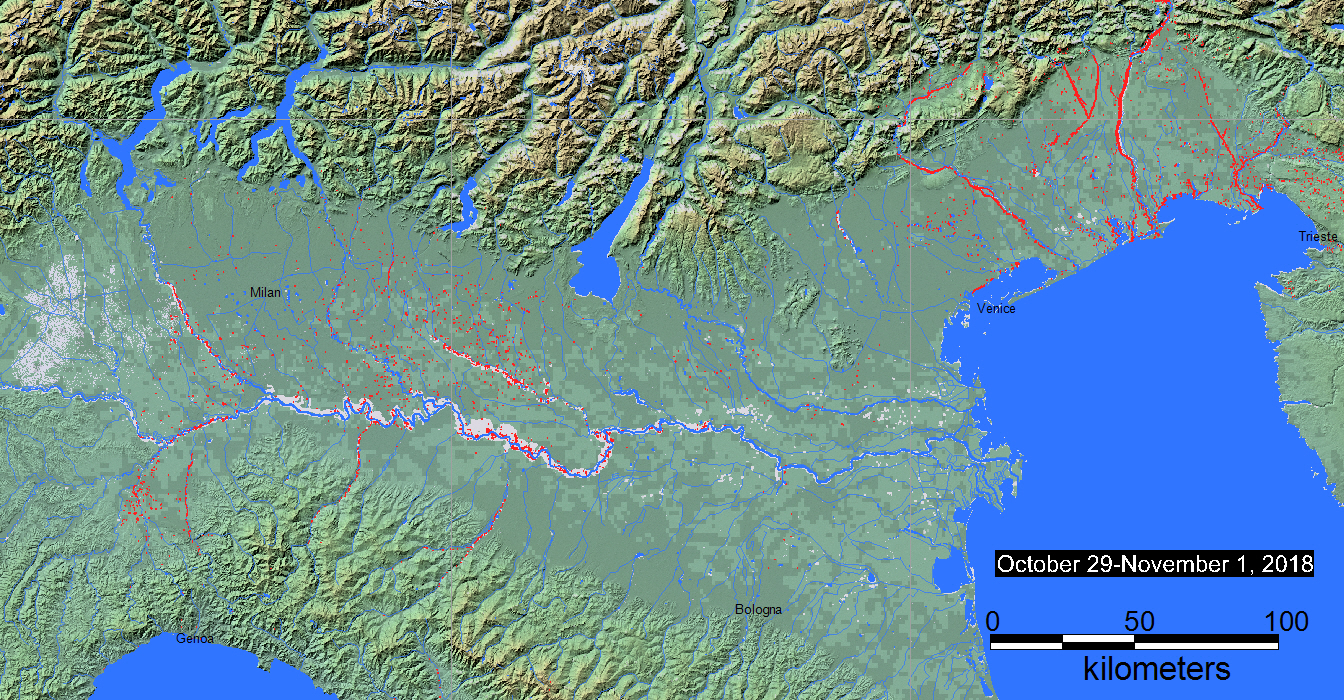
\includegraphics[width=\textwidth]{figures/ita_flood/2018Italy4699}
    \decoRule
    \caption[Flooded area in the November 2018 Italian flood]{
        Flooded areas in Northern Italy for the November 2018 event, from the DFO archive (DFO event number 4699). Blue is reference water extent, grey is maximum water extent in the archive, and red is peak flooding for this event. Image from \url{http://floodobservatory.colorado.edu/Events/4699/2018Italy4699.html}.
} \label{fig:DFO_flood_nov18}
\end{figure}

\begin{figure}
    \centering
    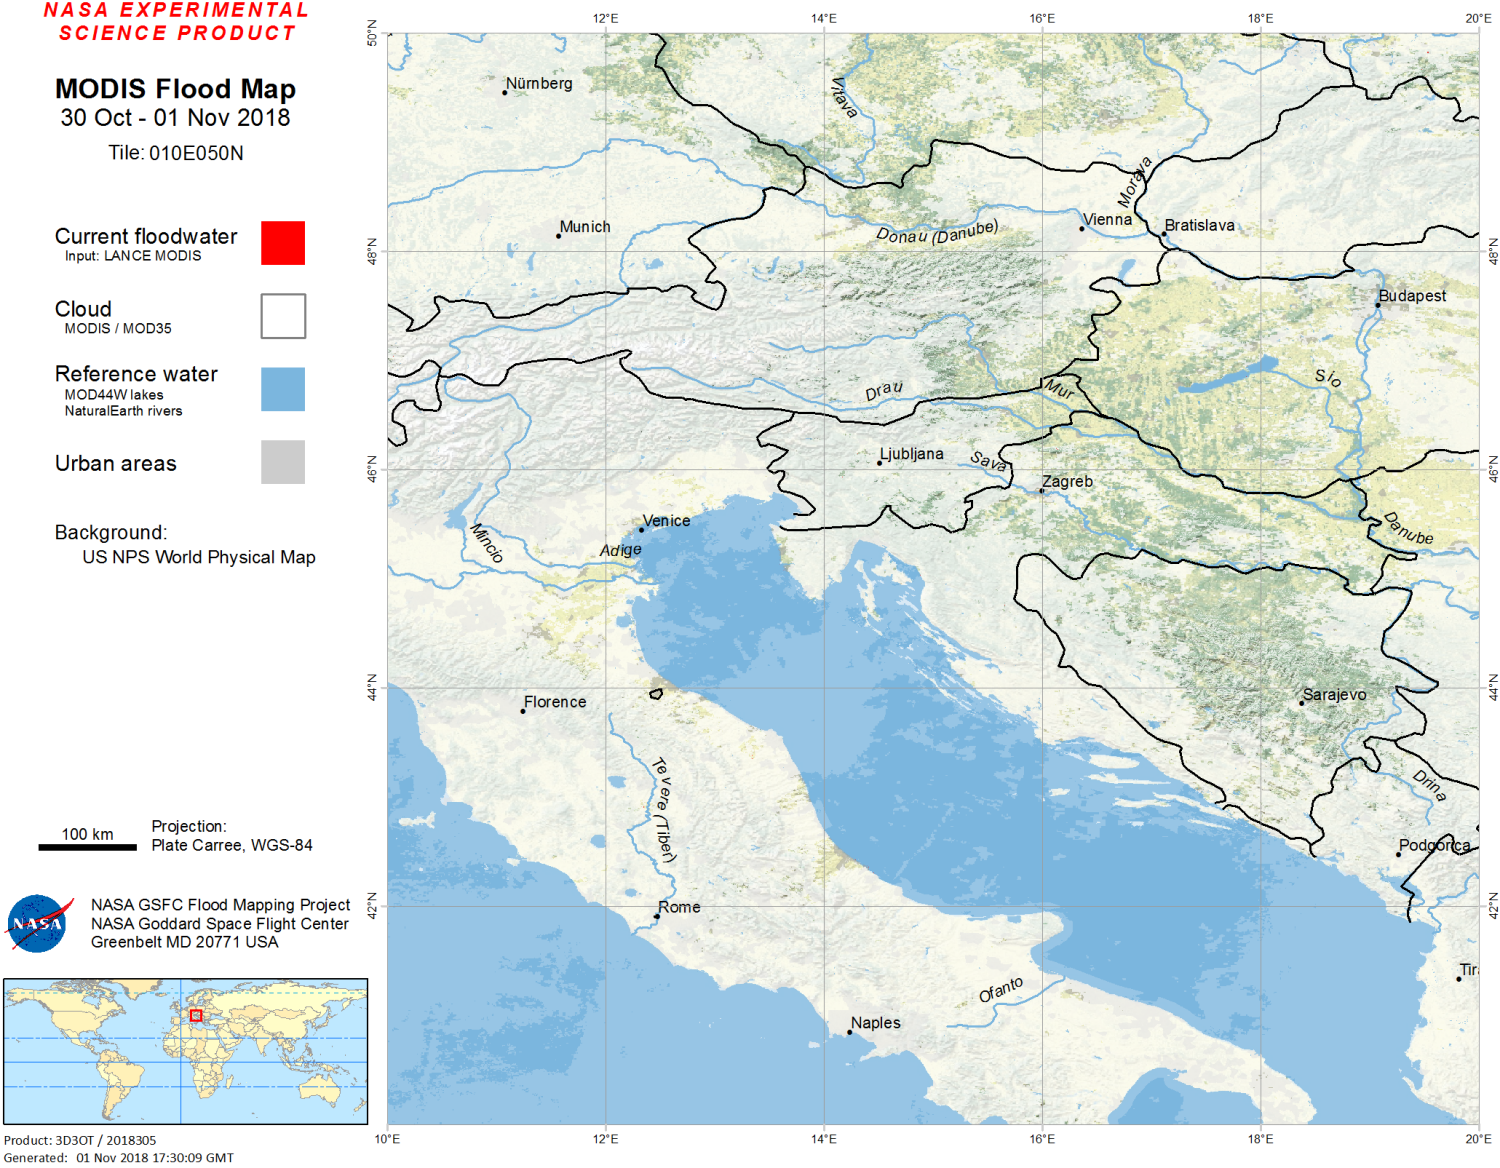
\includegraphics[width=\textwidth]{figures/ita_flood/MFM_2018305_010E050N_3D3OT}
    \decoRule
    \caption[Flooded area in the November 2018 Italian flood]{
        Flooded areas (or absence thereof) in North-Eastern Italy for the November 2018 event from the MODIS NASA NRT Global Flood Mission . Image from \url{https://floodmap.modaps.eosdis.nasa.gov/getTile.php?location=010E050N&day=305&year=2018&product=3}.
} \label{fig:NRT_flood_nov18}
\end{figure}

Several challenges in flood mapping still need to be overcome in order to provide reliable flood extent dataset for all major events. For example, small rivers often cannot be mapped or are severely underestimated by satellites due to the shielding effect of vegetation \citep{SMITH1997}; algorithm details and calibration also add an additional level of uncertainty which is often difficult to quantify \citep{Stephens2012}.\\
Due to these challenges, the current focus of companies and research scientists seems to be mainly on near-real-time flood monitoring, short-term forecasting and long-term flood hazard mapping, rather than on validation of specific events. As such, few detailed observations of flood events are available over the Italian territory; tools such as the Aqueduct Global Flood Analyzer \citep{Luo2015} from the World Resources Institute, the Web Portal from DFO\footnote{\url{https://diluvium.colorado.edu/arcgis/apps/Viewer/index.html?appid=759d697577dd438ab7f2d48f605593d5}} and the Global Surface Water Explorer \citep{Pekel2016} from the European Joint Research Centre focus mainly on long-term flood hazard mapping and/or large scale events only.
The Copernicus Global Flood Awareness System \citep[GLOFAS][]{Alfieri2013}, instead, provides daily flood extents and short-term flood forecasts. The COSMO-SkyMed stellite constellation \citep{Covello2010} has been used for evaluation of specific flood events \citep[see e.g.][]{Refice2014, Pierdicca2013, Pulvirenti2011}, but the data availability seems to be limited. In short, very little information is currently available to validate inundation models against specific events over Italy: in this work, information from all of the above sources was taken into account and used when possible, given the above mentioned caveats.


%------------------------------------
%	DEM OBS
%------------------------------------
\section{Elevation observations} \label{sec:DEM}
Elevation information for each location in the study area is necessary for the hydrological (CHyM, \cref{sec:chym}) and hydraulic (CA-2D, \cref{sec:ca2d}) models: the former uses elevation to reconstruct a realistic river network; the latter, instead, uses it to know where and how water can propagate in case of flooding. For both of these applications, high vertical accuracy, proper river routing and high horizontal resolution are necessary.

Satellite-based remote sensing techniques are the most common source of elevation data over the whole globe. Several publicly available datasets, such as SRTM, ASTER, TanDEM-X, GTOPO30 and AW3D30 use satellite sensing to infer terrain elevation and provide world coverage at resolutions ranging from \SI{30}{\metre} to \SI{1}{\kilo\metre}. Due to the nature of remote sensing via satellite, all of these datasets are affected by relatively large errors in the elevation, with vertical accuracies often of the order of several tens of meters. This makes them unsuitable for flood mapping especially of smaller basins and in flatlands.\\
A possible alternative is represented by datasets obtained by scanning the Earth's surface via LiDAR-equipped planes: these datasets, albeit very accurate, are usually very expensive for the end user (upwards of \SI{10}[\$]{\per\km\squared}), especially if a large area is required.\\
A third option for hydrologists and flood modellers is to use specifically conditioned Digital Surface Models (the term is sometimes used interchangeably with Digital Elevation Models, or DEMs) which include information on the position and depth of rivers. This is the course taken within this thesis work.

\subsection{The HydroSHEDS Digital Elevation Model}
In this thesis, the HydroSHEDS\footnote{Hydrological data and maps based on SHuttle Elevation Derivatives at multiple Scales} dataset  \citep{Lehner2008, Lehner2013} was selected to provide information not only about elevation data, but also river network and river depth. HydroSHEDS is based on different versions of NASA's 3 arc-second (about \SI{90}{\metre} at the equator) SRTM satellite-based elevation data, with several other datasets used for control and void filling. Being a DSM, and not a DTM (Digital Terrain Model), HydroSHEDS, like most satellite-only products, is affected by surface features such as buildings, major roadways and vegetation.
The DEM is hydrologically conditioned to reproduce river networks all over the globe using a mixture of automatic and manual techniques. In particular, the following algorithms are applied in order:

\begin{description}
    \item[Deepening of open water surfaces] Open waters such as lakes and oceans are deepened to insure proper flow towards them.
    \item[Weeding of coastal zone] Coastal areas are lowered to account for higher vegetation  height near the sea.
    \item[Stream burning] Major river courses are carved into the surface to ensure proper river flow. A \SI{500}{\metre} buffer is also carved around rivers to avoid sudden elevation changes and shape a smoother transition between the rivers and the surrounding areas.
    \item[Filtering] Local filtering with a $3 \times 3$ kernel size to remove high points blocking the flow path.
    \item[Molding of valley courses] Additional local algorithm to identify valley direction, using a $5 \times 5$ kernel.
    \item[Sink filling] Filling of non-natural sinks  which can impede river flow.
    \item[Carving through barriers] Final step to ensure continuous flow through natural (e.g.\ lakes) and man-made (e.g.\ dams) objects.
    \item[Second conditioning] After the barrier carving procedure, second application of the first six conditioning steps.
\end{description}

HydroSHEDS is particularly suited to the creation of a reliable river network for the CHyM model (see \cref{sec:chym_riv_net}), resulting in higher accuracy compared to the default \SI{300}{\metre} Italian DEM that comes with the model. Additionally, an advantage of using a global DEM is that it is easy to extend the flood mapping procedure to any area of the world, without the need to have any additional data requirement.\\
At the time of writing, the CHyM model is also being tested for running directly on the HydroSHEDS river network, without any further conditioning procedure as carried out by the model by default.

HydroSHEDS comes as ESRI binary \texttt{.bil} files, and was converted to appropriate formats to use with our models (NetCDF for CHyM and ASCIIgrid for CA2D) using GDAL's \texttt{gdal\_translate} tool \citep{GDAL}.

\subsection{Alternative elevation models}
Several DEMs are publicly available under no fee for research use, both for specific regions and with worldwide extent. \Cref{tab:DEMs} shows a non-comprehensive list of commonly-used DEMs, with their availability, references and maximum resolution.
\begin{sidewaystable}[]
\centering
\begin{tabular}{@{}m{2.5cm}lm{2.2cm}m{2.4cm}m{5cm}m{2.1cm}m{5cm}@{}}
\toprule
DEM name & Region & Provider & Resolution & Data source & Coordinate system & Reference \\ \midrule

PCN20 & Italy & Italian ministry for the environment & \SI{20}{\metre} & Contour lines from Italian Military Geographic Institute (IGM) cartography & UTM 32N EPSG:32632 & Provider site \footnote{\url{http://www.pcn.minambiente.it}} \\

TINITALY/01 & Italy & INGV & \SI{10}{\metre} & Mixed: satellite, cartography, LiDAR, ground data & UTM 32N EPSG:32632 & \citet{Tarquini2007, Tarquini2012} \footnote{\url{http://tinitaly.pi.ingv.it/}} \\

ASTER GDEM-2 & World & NASA & \SI{1}{arc-second} (about \SI{30}{\metre}) & Satellite & Lat-Lon EPSG:4326 & Provider site \footnote{\url{https://asterweb.jpl.nasa.gov/gdem.asp}} \\

SRTM & World  & NASA & \SI{1}{arc-second} (about \SI{30}{\metre}) & Satellite & Lat-Lon EPSG:4326 & Provider site \footnote{\url{https://www2.jpl.nasa.gov/srtm/}} \\

EU-DEM & Europe & EEA & \SI{25}{\metre} & SRTM and ASTER & EPSG:3035 ETRS89-LAEA & \citet{Bashfield2011,Jozsa2014} \footnote{\url{https://www.eea.europa.eu/data-and-maps/data/copernicus-land-monitoring-service-eu-dem}} \\

TanDEM-X & World & DLR & \SI{90}{\metre} (free version) & Satellite & Lat-Lon EPSG:4326 & \citet{Rizzoli2017}\footnote{\url{https://geoservice.dlr.de/web/dataguide/tdm90/}} \\

ALOS World 3D (AW3D30) & World & JAXA & \SI{1}{arc-second} (about \SI{30}{\metre}) & Satellite & Lat-Lon EPSG:4326 & \citet{Tadono2016, Tadono2017} \footnote{\url{https://www.eorc.jaxa.jp/ALOS/en/aw3d30/index.htm}} \\

GTOPO30 & World  & USGS & \SI{30}{arc-second} (about \SI{1}{\kilo\metre}) & Satellite & Lat-Lon EPSG:4326 & \citet{USGS1996} \footnote{\url{https://lta.cr.usgs.gov/GTOPO30}} \\

HYDRO1K & World & USGS & \SI{30}{arc-second} (about \SI{1}{\kilo\metre}) & GTOPO30, hydrologically conditioned. Flow directions and river information available & Lat-Lon EPSG:4326 & \citet{USGS1996} \footnote{\url{https://lta.cr.usgs.gov/HYDRO1K}} \\

HydroSHEDS & World  & WWF  & \SI{3}{arc-second} (about \SI{90}{\metre})   & SRTM, hydrologically conditioned. Flow directions and river information available & Lat-Lon EPSG:4326 & \citet{Lehner2008, Lehner2013} \footnote{\url{https://www.hydrosheds.org}} \\ \bottomrule
\end{tabular}\caption[List of DEMs over Italy]{Non comprehensive overview of some free-to-use DEMs and DTMs available over Italy.}\label{tab:DEMs}
\end{sidewaystable}

\begin{figure}
    %DEM difference tests: /home/clima-archive4-b/afantini/DEM/test_difference2/
    \centering
    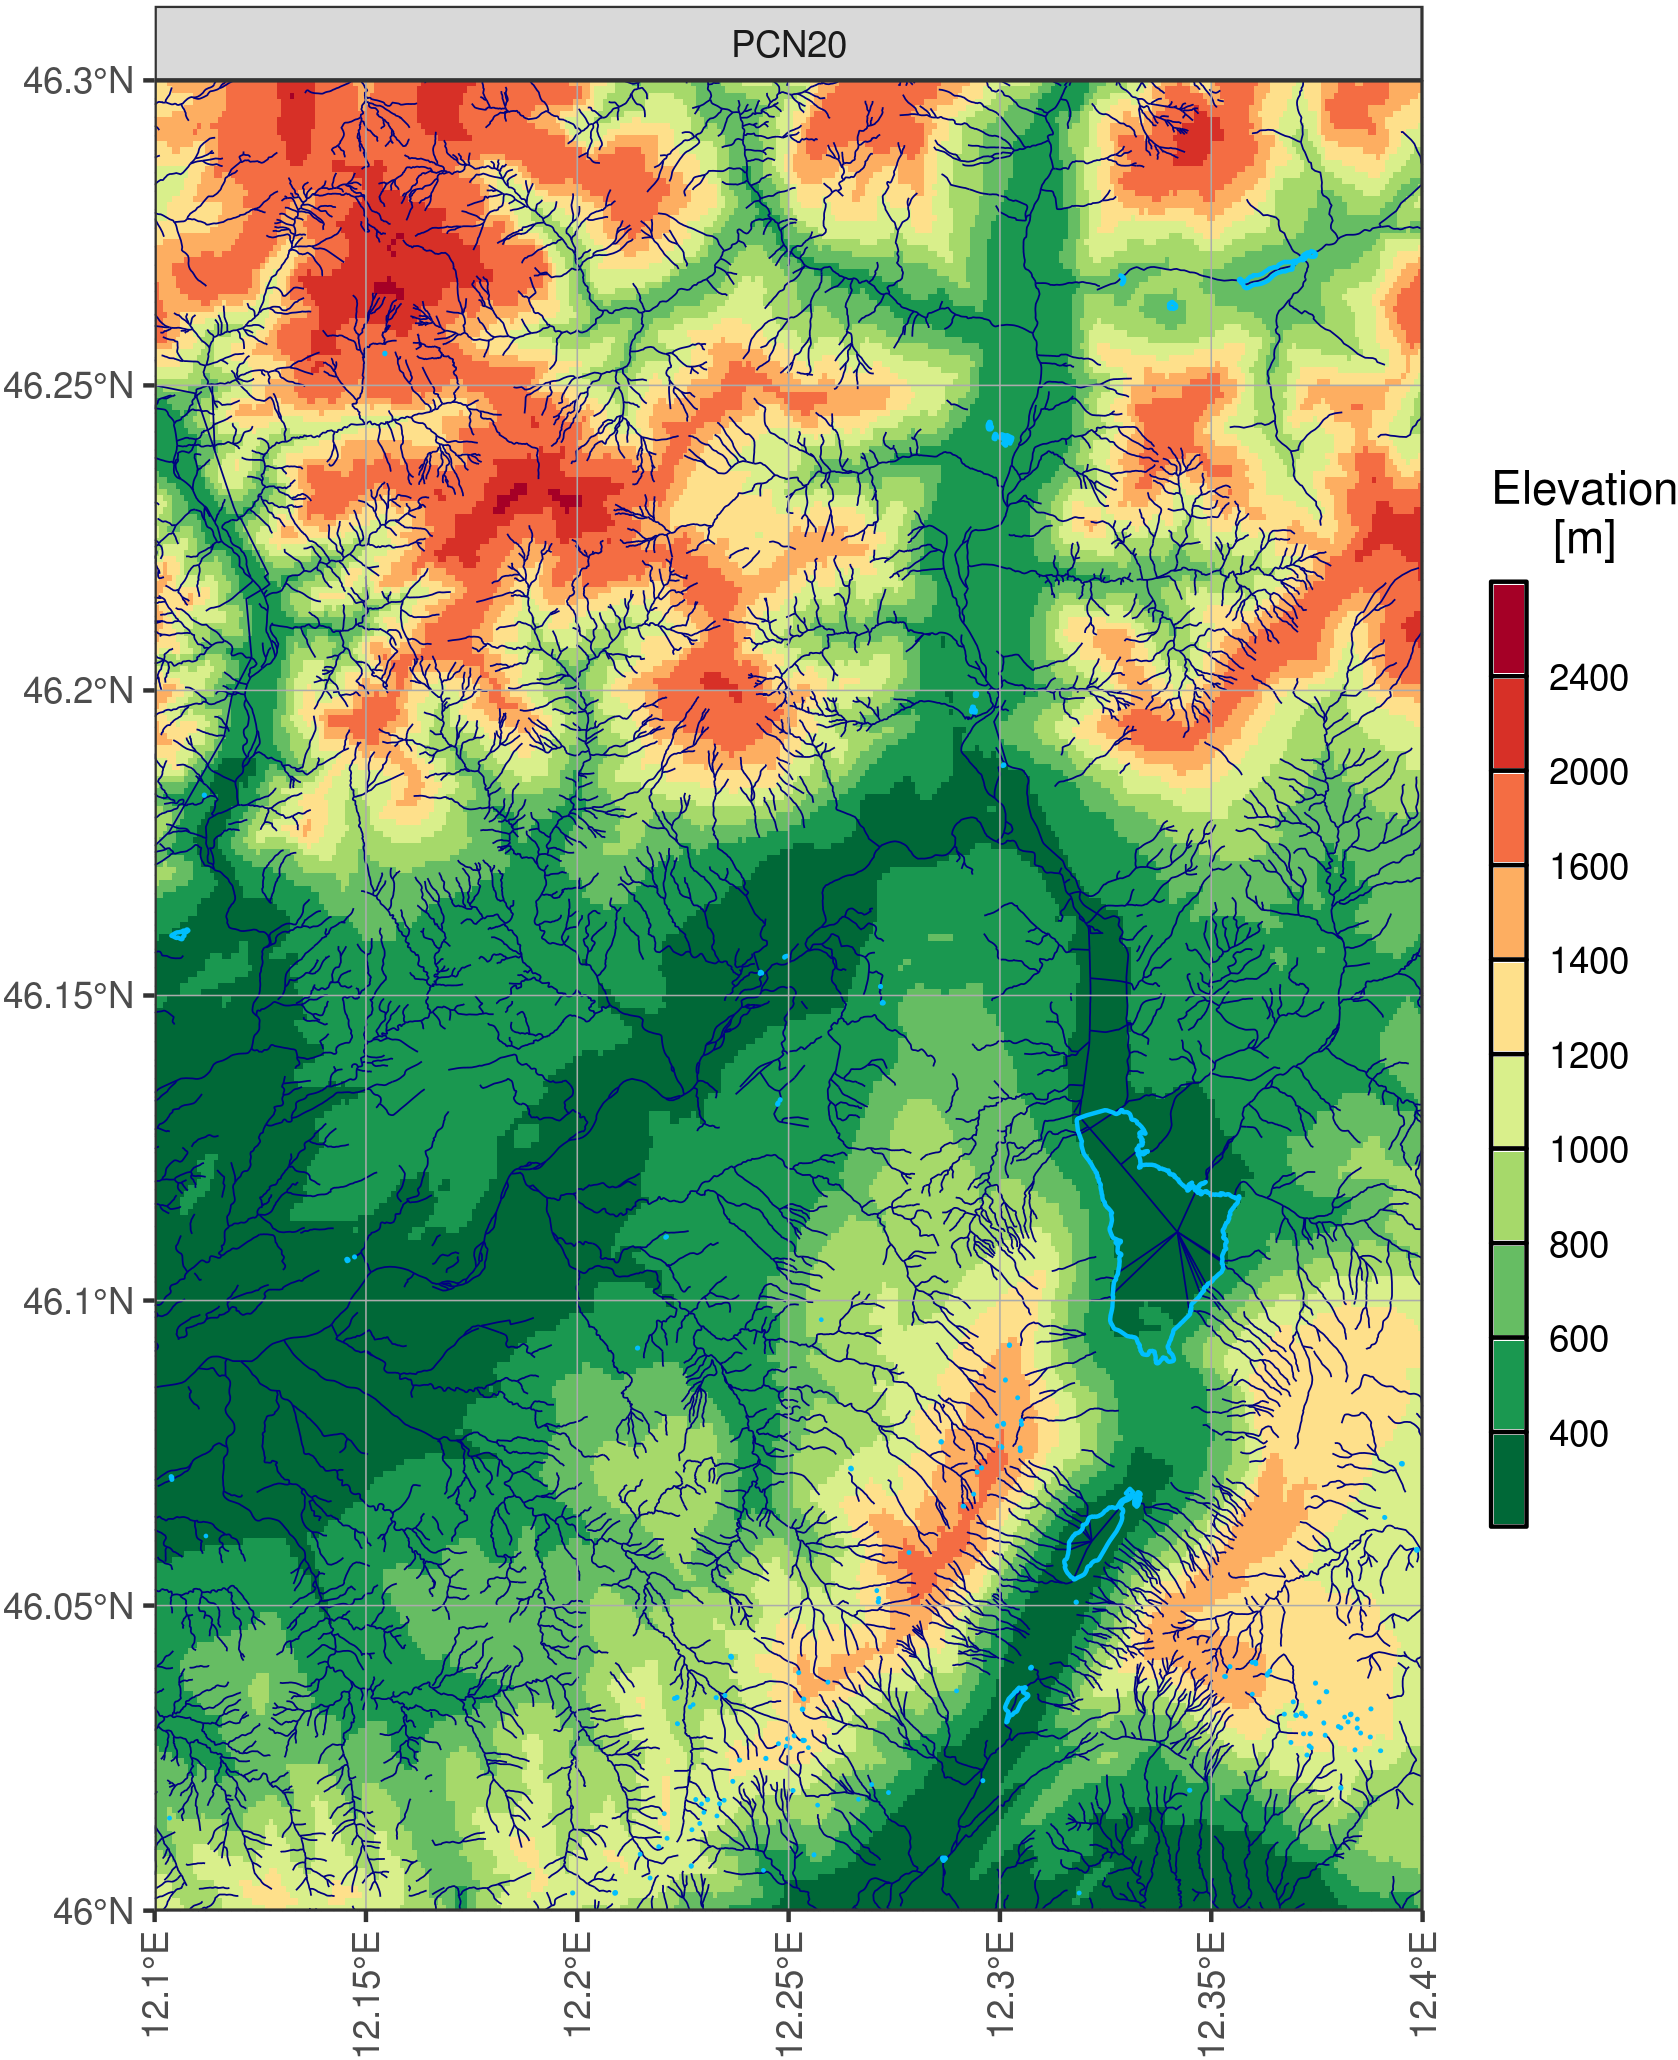
\includegraphics[width=0.5\textwidth]{figures/DEM/PCN20.png}
    \decoRule
    \caption[Comparison of DEMs: PCN20]{
    Elevation of the Italian PCN DEM at \SI{20}{\metre} resolution; detail of a selected North-Eastern Italian region centred around the town of Belluno. Rivers (dark blue) and lakes (bright blue) are from the Interregional Centre for Information, Geographical and Statistical Systems (CISIS) DBPrior10K project\footnote{\url{http://www.centrointerregionale-gis.it/DBPrior/DBPrior.html}}.
    }
    \label{fig:PCN20}
\end{figure}
In \cref{fig:PCN20} and \ref{fig:DEMs_bias}, six of them are compared for a small ($\ang{0.3}\times\ang{0.3}$) mountainous region in North-Eastern Italy, with reference to the Italian official PCN20 \SI{20}{\metre} DEM (whose elevation is displayed in \cref{fig:PCN20}). 
The region of choice, centred around the town of Belluno, includes deep valleys, a major lake towards the East and a large river (for the standards of the region) flowing through from North towards South-West.
\Cref{tab:DEMs_stats} shows mean, standard deviation, median and 5--95\% quantile ranges for the bias with the reference dataset. Large variations of up to several tens of meters can be found between the datasets (\cref{fig:DEMs_bias}); additionally, one dataset (Nasa's SRTM) shows large no-data regions which would need to be filled in before usage with a hydrological model was possible. The conditioned version of HydroSHEDS is, on average, several meters deeper than the other datasets (\SI{18.4}{\metre} deeper than the non-conditioned version), with a 5--95\% bias quantile range of \SIrange{-86}{29}{\metre}, the widest among those considered. Carved flow paths are evident along the main course of the river and in the largest lake.

\begin{figure}
    \centering
    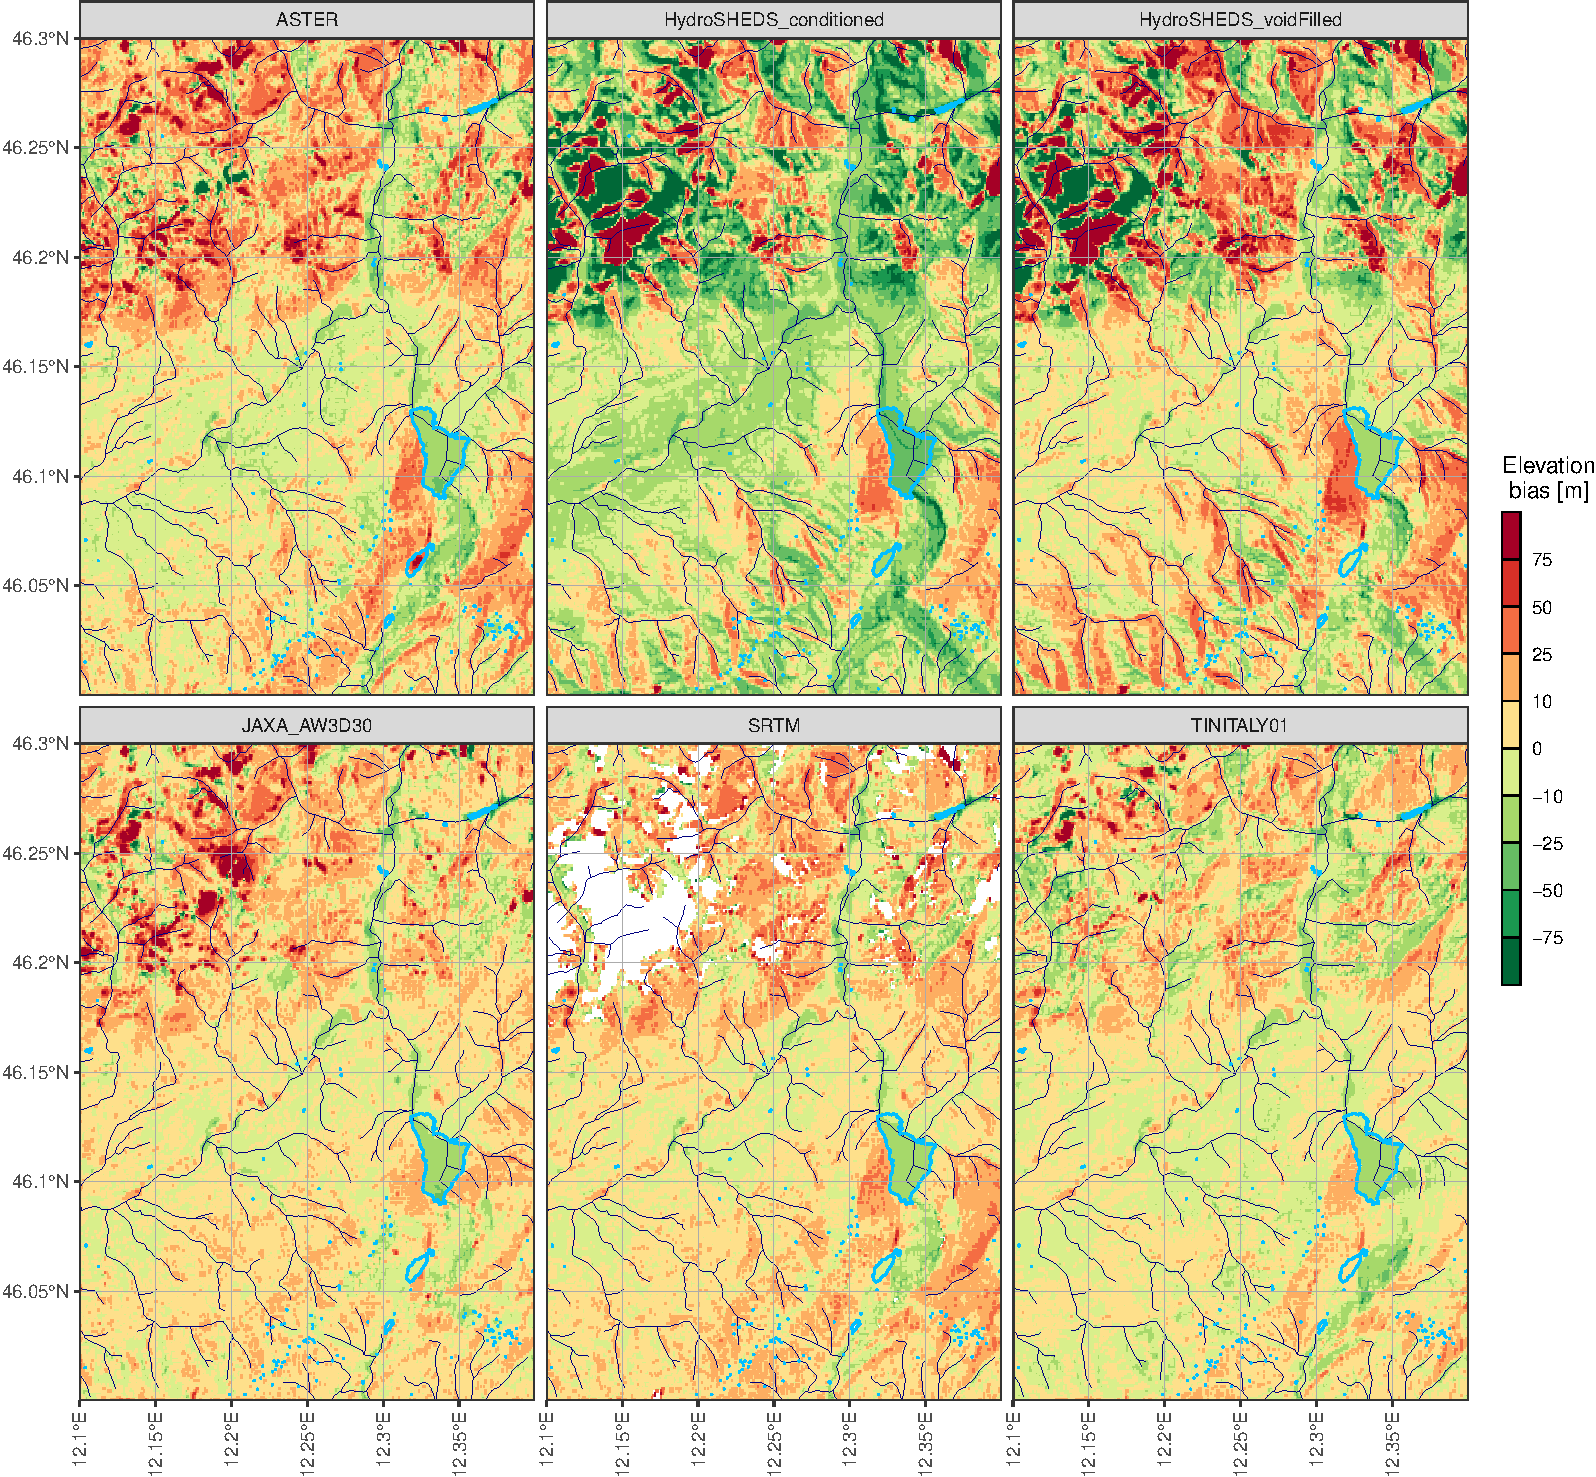
\includegraphics[width=\textwidth]{figures/DEM/bias_with_PCN20.pdf}
    \decoRule
    \caption[Comparison of DEMs: bias with PCN20]{
    Example comparison of 6 DEMs (see \cref{tab:DEMs}) over a small region in North-Eastern Italy centred around the town of Belluno. Elevation biases are calculated with reference to the national PCN20 DEM displayed in \cref{fig:PCN20}. Red means the DEM is higher than PCN20, green indicates the opposite. For the purpose of this example, all grids were warped to a common $300 \times 300$ $\ang{0.001}$ resolution grid using bilinear resampling. Overlaid simplified rivers (dark blue) are obtained from the Italian Superior Institute for the Ambient Protection and Research (ISPRA) online catalogue SINAnet\footnote{\url{http://www.sinanet.isprambiente.it/it/sia-ispra/download-mais/reticolo-idrografico/view}}; lakes (bright blue) are the same as \cref{fig:PCN20}.
} \label{fig:DEMs_bias}
\end{figure}

\begin{table}[]
\centering
\begin{tabular}{@{}llllll@{}}
\toprule
DEM                     & Mean   & StdDev & Q05   & Median & Q95 \\ \midrule
ASTER                   & 3.9    & 30.1   & -21   & 1      & 36 \\
HydroSHEDS Void Filled  & 0.4    & 57.8   & -52   & 0      & 51 \\
HydroSHEDS VF + Cond.  & -16.4  & 59.7   & -86   & -11    & 29 \\
JAXA AW3D30             & 5.0    & 19.6   & -14   & 3      & 26 \\
SRTM                    & 4.7    & 14.1   & -14   & 3      & 25 \\
TINITALY/01              & -0.6   & 14.1   & -19.3 & -0.6   & 17.7   
\end{tabular}
\decoRule
\caption[Comparison of DEMs: bias metrics with PCN20]{Statistics for the DEM comaparison of \cref{fig:DEMs_bias}. All values are in meters.} \label{tab:DEMs_stats}
\end{table}

In general, the choice of Digital Elevation Model must be driven by the project's requirements, and not by average bias. In this case, a reliable river network representation was paramount, leading us to settle with HydroSHEDS as terrain model of choice. Other global and regional elevation datasets were tested by attempting to reconstruct a reasonable river network via the hydrological model CHyM (\cref{sec:chym_riv_net}), but none allowed to reconstruct the rivers as well as the hydrologically conditioned HydroSHEDS.
